% !TeX root = ../main.tex
\section{Mô tả sản phẩm/dịch vụ}

% !TeX root = ../main.tex
\subsection{Giải pháp đưa ra}

Dự án đề xuất xây dựng một nền tảng web/app cho phép người dùng \textbf{thuê thiết bị gaming trong vài ngày hoặc thử trước khi mua}. Người dùng có thể tìm kiếm thiết bị theo loại sản phẩm, thương hiệu, game phù hợp, giá thuê, tình trạng thiết bị và thông số kỹ thuật. Sau đó, người dùng đặt thuê, thanh toán phí thuê và chọn một trong hai cách bảo chứng: đặt cọc truyền thống hoặc đăng ký hỗ trợ cọc, rồi nhận thiết bị để trải nghiệm thực tế.

Về dòng tiền, Mutux đóng vai trò trung gian giữa người thuê và người cho thuê. Với cách thuê truyền thống, người thuê thường phải trả cùng lúc \textbf{tiền thuê} và \textbf{tiền cọc tương đương toàn bộ giá trị sản phẩm}. Đây là rào cản lớn vì ngay cả một món gear có giá dưới 2.000.000 đồng, người thuê vẫn phải chuẩn bị gần như đủ giá trị món hàng làm tiền cọc, sau đó mới trả thêm tiền thuê cho lần mượn đó.

Với giải pháp của Mutux, người thuê không cần bỏ ra một khoản lớn như vậy cho một lần thuê. Nền tảng có thể hỗ trợ hoặc kết nối đối tác tài chính để \textbf{cho vay phần cọc}, với hạn mức phụ thuộc vào giá trị sản phẩm và mức độ xác minh của người thuê. Khi đặt thuê, người thuê chỉ cần trả \textbf{tiền thuê do người cho thuê đặt ra} cộng với một \textbf{khoản phí vay/hỗ trợ cọc nhỏ}, thường rẻ tương tự cách các ví trả sau hoặc SPayLater tính phí cho khoản trả sau ngắn hạn. Nhờ đó, phần cọc vẫn được bảo chứng để xử lý trường hợp hư hỏng hoặc mất thiết bị, nhưng người thuê không phải khóa một số tiền lớn ngay từ đầu.

\begin{figure}[h!]
    \centering
    \begin{tikzpicture}[
        box/.style={
            draw=primary,
            rounded corners=4pt,
            line width=0.8pt,
            align=center,
            minimum width=3.0cm,
            minimum height=1.1cm,
            fill=primary!5
        },
        smallbox/.style={
            draw=accent,
            rounded corners=4pt,
            line width=0.8pt,
            align=center,
            minimum width=3.5cm,
            minimum height=0.95cm,
            fill=accent!7
        },
        flow/.style={-{Latex[length=2.5mm]}, line width=0.75pt, color=secondary},
        money/.style={-{Latex[length=2.5mm]}, line width=0.9pt, color=accent},
        note/.style={align=center, font=\footnotesize}
    ]
        \node[box] (renter) at (0,1.8) {Người thuê\\game gear};
        \node[box] (platform) at (5.5,1.8) {Nền tảng\\Mutux};
        \node[box] (owner) at (11.0,1.8) {Người cho thuê\\shop/chủ gear};
        \node[smallbox] (deposit) at (5.5,-0.4) {Bảo chứng cọc\\xử lý hư hỏng/mất thiết bị};

        \draw[money] ([yshift=0.26cm]renter.east) -- ([yshift=0.26cm]platform.west)
            node[midway, above=0.12cm, note, text width=3.2cm]{Truyền thống: cọc 100\% giá trị + phí thuê};
        \draw[money] ([yshift=-0.26cm]renter.east) -- ([yshift=-0.26cm]platform.west)
            node[midway, below=0.12cm, note, text width=3.2cm]{Mutux: phí thuê + phí vay cọc nhỏ};
        \draw[money] ([yshift=0.26cm]platform.east) -- ([yshift=0.26cm]owner.west)
            node[midway, above=0.12cm, note, text width=3.2cm]{Tiền thuê sau hoa hồng};
        \draw[money] (platform.south) -- (deposit.north)
            node[midway, right=0.12cm, note]{quản lý cọc};

        \draw[flow] (11.0,-2.4) -- (0,-2.4)
            node[midway, above=0.12cm, note]{Giao thiết bị};
        \draw[flow] (0,-3.0) -- (11.0,-3.0)
            node[midway, below=0.12cm, note]{Trả thiết bị};
    \end{tikzpicture}
    \caption{Luồng thiết bị và dòng tiền trong mô hình Mutux}
\end{figure}

\subsubsection{Các loại thiết bị có thể cho thuê}

\begin{itemize}
    \item Chuột gaming: Logitech, Razer, Zowie, Pulsar, Lamzu, Glorious.
    \item Bàn phím cơ: phân loại theo layout, switch, kết nối và độ phản hồi.
    \item Tai nghe gaming: test âm thanh, mic, độ thoải mái khi đeo lâu.
    \item Tay cầm: phục vụ FC Online, eFootball, FIFA, PES, racing game.
    \item Combo gear: chuột, bàn phím và tai nghe theo từng thể loại game.
\end{itemize}

\subsubsection{Tính năng cho người thuê}

\begin{itemize}
    \item Đăng ký và đăng nhập tài khoản.
    \item Xem danh sách thiết bị gaming đang có sẵn.
    \item Lọc thiết bị theo loại, thương hiệu, giá thuê, tình trạng và game phù hợp.
    \item Xem chi tiết thiết bị gồm ảnh, thông số, mô tả, tình trạng và đánh giá.
    \item Đặt thuê theo ngày.
    \item Thanh toán phí thuê, đặt cọc hoặc đăng ký hỗ trợ cọc.
    \item Theo dõi trạng thái đơn thuê.
    \item Đánh giá thiết bị sau khi trả hàng.
    \item Nhận gợi ý gear phù hợp theo game đang chơi.
\end{itemize}

\subsubsection{Tính năng cho shop hoặc chủ gear}

\begin{itemize}
    \item Đăng thiết bị lên nền tảng.
    \item Quản lý danh sách thiết bị.
    \item Cập nhật tình trạng thiết bị: available, booked, renting, returned, maintenance.
    \item Quản lý lịch thuê.
    \item Theo dõi doanh thu.
    \item Xem đánh giá từ người thuê.
\end{itemize}

\subsubsection{Tính năng cho admin}

\begin{itemize}
    \item Quản lý người dùng.
    \item Quản lý thiết bị.
    \item Quản lý đơn thuê.
    \item Kiểm duyệt thiết bị do shop hoặc chủ gear đăng.
    \item Xử lý tranh chấp, trả muộn, hư hỏng hoặc mất thiết bị.
    \item Theo dõi doanh thu và hoa hồng nền tảng.
\end{itemize}


% !TeX root = ../main.tex
\subsection{Mô tả sản phẩm và dịch vụ}

\subsubsection{Tổng quan về sản phẩm và dịch vụ}
    Nhóm phát triển một nền tảng trực tuyến chuyên cung cấp dịch vụ cho thuê Gear công nghệ, bao gồm bàn phím cơ, tai nghe, tay cầm chơi game và nhiều thiết bị ngoại vi khác. Với thông điệp ``Trải nghiệm Gear xịn, không cần chi phí lớn'', nền tảng giúp sinh viên và người dùng trẻ dễ dàng tiếp cận những sản phẩm chất lượng cao mà không phải chịu áp lực tài chính khi mua mới.

    Thông qua website, khách hàng có thể tìm kiếm và so sánh thiết bị, lựa chọn thời gian thuê, đặt lịch và thanh toán trực tuyến một cách nhanh chóng, thuận tiện. Không chỉ phục vụ người thuê, nền tảng còn kết nối các cửa hàng Gear nhỏ lẻ với cộng đồng yêu công nghệ, tạo thêm một kênh kinh doanh hiệu quả. Qua đó, các đối tác có thể mở rộng tệp khách hàng, gia tăng tần suất khai thác sản phẩm và tối ưu doanh thu từ nguồn thiết bị sẵn có.

\subsubsection{Vấn đề của khách hàng mà sản phẩm giải quyết}
    Nhiều người dùng mong muốn trải nghiệm cảm giác gõ khác biệt của một chiếc bàn phím cơ cao cấp, chất âm sống động từ tai nghe chất lượng hay độ phản hồi chính xác của tay cầm chuyên nghiệp. Tuy nhiên, mức giá cao cùng nỗi lo mua nhầm sản phẩm không phù hợp khiến họ ngần ngại đầu tư.

    Nền tảng của nhóm giải quyết những rào cản này bằng mô hình ``thuê để trải nghiệm''. Người dùng có thể sử dụng Gear cao cấp với chi phí hợp lý, thử nghiệm sản phẩm trong điều kiện thực tế và đưa ra quyết định mua sắm tự tin hơn. Giải pháp đặc biệt phù hợp với sinh viên, game thủ trẻ, người sáng tạo nội dung và những người yêu công nghệ có nhu cầu sử dụng thiết bị trong thời gian ngắn.

    Ở phía đối tác, nhiều cửa hàng Gear nhỏ lẻ vẫn phụ thuộc vào lượng khách trực tiếp, phạm vi tiếp cận hạn chế và chưa khai thác tối đa giá trị của hàng trưng bày hoặc thiết bị sẵn có. Thông qua nền tảng, các cửa hàng có thể tiếp cận nhiều khách hàng tiềm năng hơn, tăng vòng quay khai thác sản phẩm và xây dựng thêm nguồn doanh thu từ hoạt động cho thuê.

    Nhờ đó, nền tảng tạo ra giá trị kép cho toàn bộ hệ sinh thái: khách hàng được trải nghiệm Gear chất lượng với chi phí tối ưu, trong khi các đối tác có thêm cơ hội tăng trưởng và mở rộng thị trường. Đây không chỉ là một dịch vụ cho thuê thiết bị, mà còn là cầu nối giúp trải nghiệm công nghệ cao cấp trở nên gần gũi, linh hoạt và dễ tiếp cận hơn.

\subsection{Các tính năng chính của sản phẩm}

Mutux được thiết kế như một nền tảng hai phía, kết nối người có nhu cầu thuê/thử gaming gear với shop hoặc cá nhân đang sở hữu thiết bị. Các tính năng của sản phẩm gồm: \textbf{tính năng cho khách chưa đăng nhập}, \textbf{tính năng chung cho người dùng} và \textbf{tính năng riêng} theo từng vai trò người thuê, shop/chủ gear và admin.
\subsubsection{Tính năng cho khách chưa đăng nhập}

Khách chưa đăng nhập vẫn có thể xem trước một phần nội dung của nền tảng để hiểu dịch vụ và cân nhắc đăng ký tài khoản.

\begin{itemize}
    \item Đăng ký tài khoản: cho phép khách tạo tài khoản mới để trở thành người dùng chính thức của Mutux và sử dụng các chức năng như đặt thuê, thanh toán, đánh giá hoặc đăng thiết bị.
    \item Xem danh sách thiết bị: cho phép khách xem các thiết bị gaming đang có trên nền tảng, từ đó hiểu Mutux đang cung cấp những loại gear nào như chuột, bàn phím, tai nghe, tay cầm hoặc combo gear.
    \item Xem chi tiết thiết bị: cho phép khách xem thông tin cơ bản của từng thiết bị như ảnh, mô tả, thông số, giá thuê, tình trạng và đánh giá công khai trước khi quyết định đăng ký hoặc đặt thuê.
    \item Lọc thiết bị theo nhu cầu cá nhân: giúp người dùng thu hẹp danh sách theo loại gear, thương hiệu, giá thuê, tình trạng và game phù hợp để tìm đúng thiết bị cần thử.
\end{itemize}
\subsubsection{Tính năng chung cho người dùng hệ thống}

\begin{itemize}
    \item Đăng nhập: cho phép người dùng đã có tài khoản truy cập hệ thống và sử dụng các chức năng theo vai trò như người thuê, shop/chủ gear hoặc admin.
    \item Đổi mật khẩu: cho phép người dùng thay đổi mật khẩu sau khi đăng nhập để tăng tính bảo mật cho tài khoản.
    \item Quên mật khẩu: cho phép người dùng xác minh tài khoản và thiết lập lại mật khẩu mới khi không nhớ mật khẩu cũ.
    \item Quản lý hồ sơ cá nhân: cho phép người dùng cập nhật thông tin như họ tên, số điện thoại, email, địa chỉ nhận/trả thiết bị và thông tin xác minh cần thiết.
\end{itemize}

\subsubsection{Tính năng cho người thuê}

Các tính năng phục vụ trực tiếp quá trình người dùng tìm, thuê, trải nghiệm và quyết định có mua thiết bị hay không.

\begin{itemize}
% maybe người cho thuê cũng có thể là người thuê?
    \item Xem danh sách thiết bị: cho phép người thuê xem toàn bộ thiết bị gaming đang có trên nền tảng, bao gồm chuột, bàn phím, tai nghe, tay cầm hoặc combo gear phù hợp với nhu cầu trải nghiệm.
    \item Lọc thiết bị theo game và thông số: giúp người thuê thu hẹp danh sách theo game đang chơi, loại gear, thương hiệu, giá thuê, tình trạng hoặc các thông số kỹ thuật quan trọng khác.
    \item Đặt thuê thiết bị theo ngày: cho phép người thuê chọn số ngày thuê, thời gian nhận và trả thiết bị; hệ thống kiểm tra lịch trống để tránh đặt trùng.
    \item Thanh toán phí thuê và chọn hình thức cọc: cho phép người thuê thanh toán phí thuê theo ngày hoặc theo gói ngắn hạn, đồng thời chọn một trong hai cách bảo chứng phù hợp với khả năng tài chính:
    \begin{itemize}
        \item \textbf{Cọc truyền thống}: người thuê ứng trước tiền cọc để bảo vệ tài sản cho shop hoặc chủ gear. Khoản cọc có thể bằng toàn bộ hoặc gần toàn bộ giá trị thiết bị, không được tính là doanh thu của Mutux và sẽ được hoàn lại khi người thuê trả thiết bị đúng hạn, đúng tình trạng và đầy đủ phụ kiện.
        \item \textbf{Cọc Trả Sau/hỗ trợ cọc}: người thuê không cần khóa trước toàn bộ tiền cọc mà chỉ trả phí thuê cộng với một khoản phí vay hoặc phí bảo chứng nhỏ. Phần cọc vẫn được bảo chứng để xử lý rủi ro hư hỏng, mất thiết bị hoặc vi phạm điều kiện thuê.
    \end{itemize}
    \item Quản lý và theo dõi đơn thuê: giúp người thuê biết đơn đang ở bước nào như chờ xác nhận, đang giao, đang thuê, chờ trả hàng, đang kiểm tra hoặc hoàn tất. Người thuê có thể xem và đăng tải ảnh/video minh chứng và ghi nhận tình trạng gear ở từng mốc quan trọng gồm trước khi giao, sau khi nhận thiết bị, trước khi gửi trả, sau khi bên cho thuê nhận lại thiết bị, từ đó giảm tranh chấp về hư hỏng hoặc thiếu phụ kiện.
    \item Báo cáo đơn hàng và trao đổi với người cho thuê: cho phép người thuê báo cáo vấn đề phát sinh trong đơn như giao sai thiết bị, thiết bị không đúng mô tả, hư hỏng trước khi nhận, thiếu phụ kiện hoặc bất đồng về phí phát sinh. Người thuê cũng có thể chat trực tiếp với shop hoặc chủ gear để thống nhất thời gian giao nhận, hỏi cách sử dụng thiết bị và xử lý nhanh các tình huống trong quá trình thuê.
    \item Đăng ký gói membership: cho phép người thuê đăng ký gói thành viên để nhận ưu đãi như giảm phí thuê, giảm phí hỗ trợ cọc, ưu tiên thuê gear hot, nhận mã giảm giá giao nhận hoặc tích điểm cho các lần thuê tiếp theo.
    \item Đánh giá thiết bị sau khi trả hàng: cho phép người thuê chia sẻ cảm nhận thực tế về thiết bị sau khi sử dụng, giúp cộng đồng có thêm dữ liệu tham khảo.
    \item Đánh giá người cho thuê: cho phép người thuê chấm điểm và nhận xét shop hoặc chủ gear sau khi hoàn tất đơn dựa trên độ đúng mô tả của thiết bị, chất lượng bảo quản, thái độ hỗ trợ, tốc độ phản hồi, mức độ đúng hẹn khi giao nhận và cách xử lý vấn đề phát sinh. Các đánh giá này giúp người thuê sau lựa chọn bên cho thuê đáng tin cậy hơn, đồng thời tạo động lực để shop hoặc chủ gear mô tả thiết bị minh bạch và phục vụ tốt hơn.
    \item Xem đánh giá từ shop hoặc chủ gear: giúp người thuê biết mức độ uy tín của mình trong mắt bên cho thuê và cải thiện hành vi thuê ở các giao dịch sau.
    \item Dự định sẽ phát triển mô hình \textit{try-before-buy} trong tương lai: cho phép người thuê thử thiết bị trước, nếu hài lòng thì có thể mua sản phẩm mới từ shop đối tác hoặc mua lại chính thiết bị đang thuê nếu bên cho thuê cho phép.
\end{itemize}

\subsubsection{Tính năng cho shop hoặc chủ gear}

Nhóm tính năng này giúp shop hoặc cá nhân sở hữu gear quản lý tài sản, khai thác thiết bị nhàn rỗi và tạo thêm doanh thu từ hoạt động cho thuê.

\begin{itemize}
    \item Đăng thiết bị lên nền tảng: cho phép shop hoặc chủ gear đưa thiết bị của mình lên Mutux để người thuê có thể tìm, xem thông tin và đặt thuê.
    \item Quản lý danh sách thiết bị: cho phép bên cho thuê chỉnh sửa hình ảnh, mô tả, thông số, giá thuê, giá trị bảo chứng và các thông tin liên quan đến từng thiết bị.
    \item Quản lý đơn hàng và tình trạng thiết bị: giúp bên cho thuê theo dõi trạng thái từng đơn như chờ xác nhận, đang giao, đang thuê, chờ trả hàng, đang kiểm tra hoặc hoàn tất; đồng thời cập nhật trạng thái thiết bị để tránh nhầm lẫn khi vận hành. Shop hoặc chủ gear có thể tải lên và xem ảnh minh chứng tình trạng gear trước khi giao, sau khi người thuê nhận, trước khi người thuê trả và sau khi nhận lại thiết bị.
    \item Theo dõi và rút tiền doanh thu: giúp bên cho thuê xem doanh thu từ từng thiết bị, từng đơn thuê hoặc từng khoảng thời gian để đánh giá hiệu quả khai thác tài sản. Shop hoặc chủ gear có thể theo dõi số dư khả dụng sau khi đơn thuê hoàn tất, gửi yêu cầu rút tiền về tài khoản ngân hàng hoặc ví điện tử đã xác minh, đồng thời xem lịch sử các lần rút tiền và trạng thái xử lý như đang chờ duyệt, đã thanh toán hoặc bị từ chối.
    \item Báo cáo đơn hàng, yêu cầu bồi thường và chat với người thuê: cho phép shop hoặc chủ gear báo cáo các vấn đề như người thuê trả muộn, làm hỏng thiết bị, thiếu phụ kiện hoặc không thống nhất được tình trạng gear sau khi trả. Khi có bằng chứng phù hợp, bên cho thuê có thể gửi yêu cầu bồi thường để admin xem xét và xử lý theo quy định của nền tảng. Tính năng chat giúp hai bên trao đổi về lịch giao nhận, hướng dẫn sử dụng, nhắc trả thiết bị và giải quyết vấn đề trước khi tạo tranh chấp chính thức.
    \item Xem đánh giá từ người thuê: giúp bên cho thuê hiểu thiết bị và chất lượng phục vụ có đáp ứng nhu cầu thực tế hay không, từ đó cải thiện, bảo trì thiết bị hoặc điều chỉnh danh mục cho thuê.
    \item Đánh giá người thuê: cho phép shop hoặc chủ gear đánh giá người thuê sau khi hoàn tất đơn dựa trên việc trả hàng đúng hạn, giữ gìn thiết bị và hoàn trả đầy đủ phụ kiện.
\end{itemize}


\subsubsection{Tính năng cho admin}

Nhóm tính năng này phục vụ việc quản trị hệ thống, kiểm soát chất lượng dữ liệu và xử lý các rủi ro phát sinh trong giao dịch thuê.

\begin{itemize}
    \item Quản lý người dùng: cho phép admin xem hồ sơ, kiểm tra trạng thái và quản lý tài khoản người thuê, shop hoặc chủ gear.
    \item Quản lý thiết bị: cho phép admin theo dõi thiết bị đang đăng, phát hiện thông tin sai lệch và yêu cầu bên cho thuê chỉnh sửa.
    \item Quản lý đơn thuê: cho phép admin theo dõi trạng thái đơn, kiểm tra lịch sử giao dịch và hỗ trợ hai bên khi phát sinh vấn đề.
    \item Kiểm duyệt thiết bị: cho phép admin duyệt thông tin, hình ảnh và tình trạng thiết bị trước khi hiển thị công khai trên nền tảng.
    \item Xử lý tranh chấp: cho phép admin tiếp nhận báo cáo, xem bằng chứng giao nhận và hỗ trợ xử lý bồi thường khi có rủi ro.
    \item Theo dõi doanh thu: cho phép admin kiểm soát phí nền tảng, hoa hồng, yêu cầu rút tiền và hiệu quả vận hành kinh doanh.
\end{itemize}


\subsection{Phiên bản sản phẩm tối thiểu khả thi - MVP}

Dưới đây là User Interface ban đầu của Mutux mà nhóm sẽ thiết kế MVP.

\begin{figure}[H]
    \centering
    
    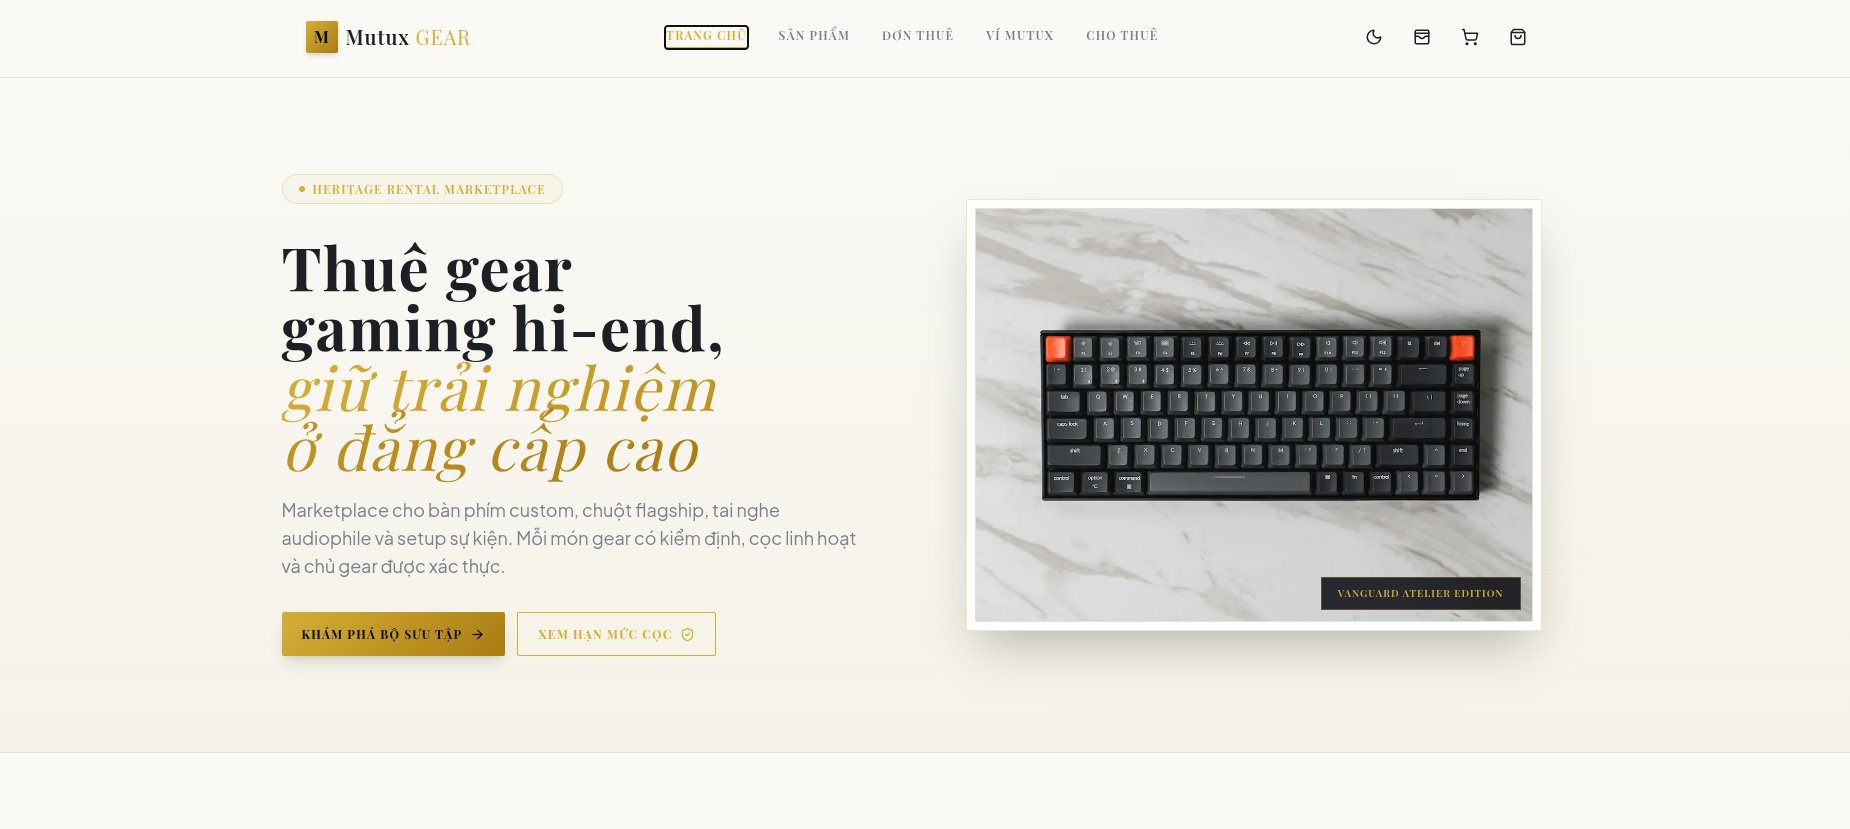
\includegraphics[width=1\textwidth]{../PA2/img/mvp/frontpage1.png}
    
    \caption{Trang chủ của Mutux}
    \label{fig:my_image} 
\end{figure}

Từ landing page này, người dùng có thể xem qua và tìm hiểu về Mutux.

\begin{figure}[H]
    \centering 
    
    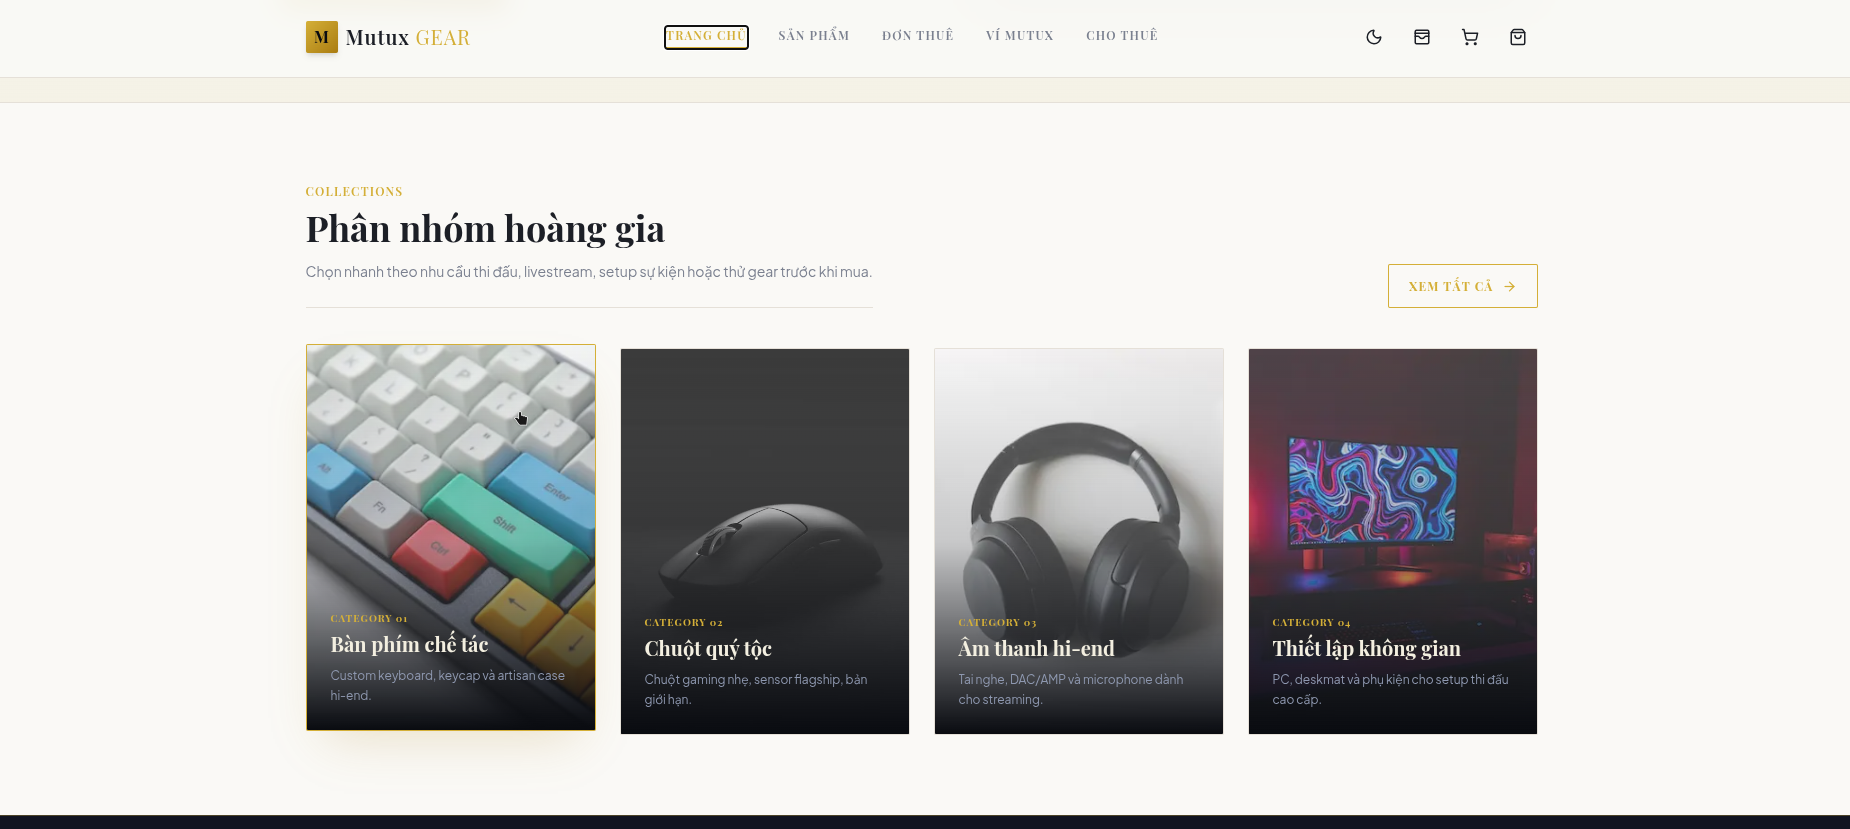
\includegraphics[width=1\textwidth]{../PA2/img/mvp/frontpage2.png}
    
    \caption{Trang chủ của Mutux}
    \label{fig:my_image}
\end{figure}

\begin{figure}[H]
    \centering 
    
    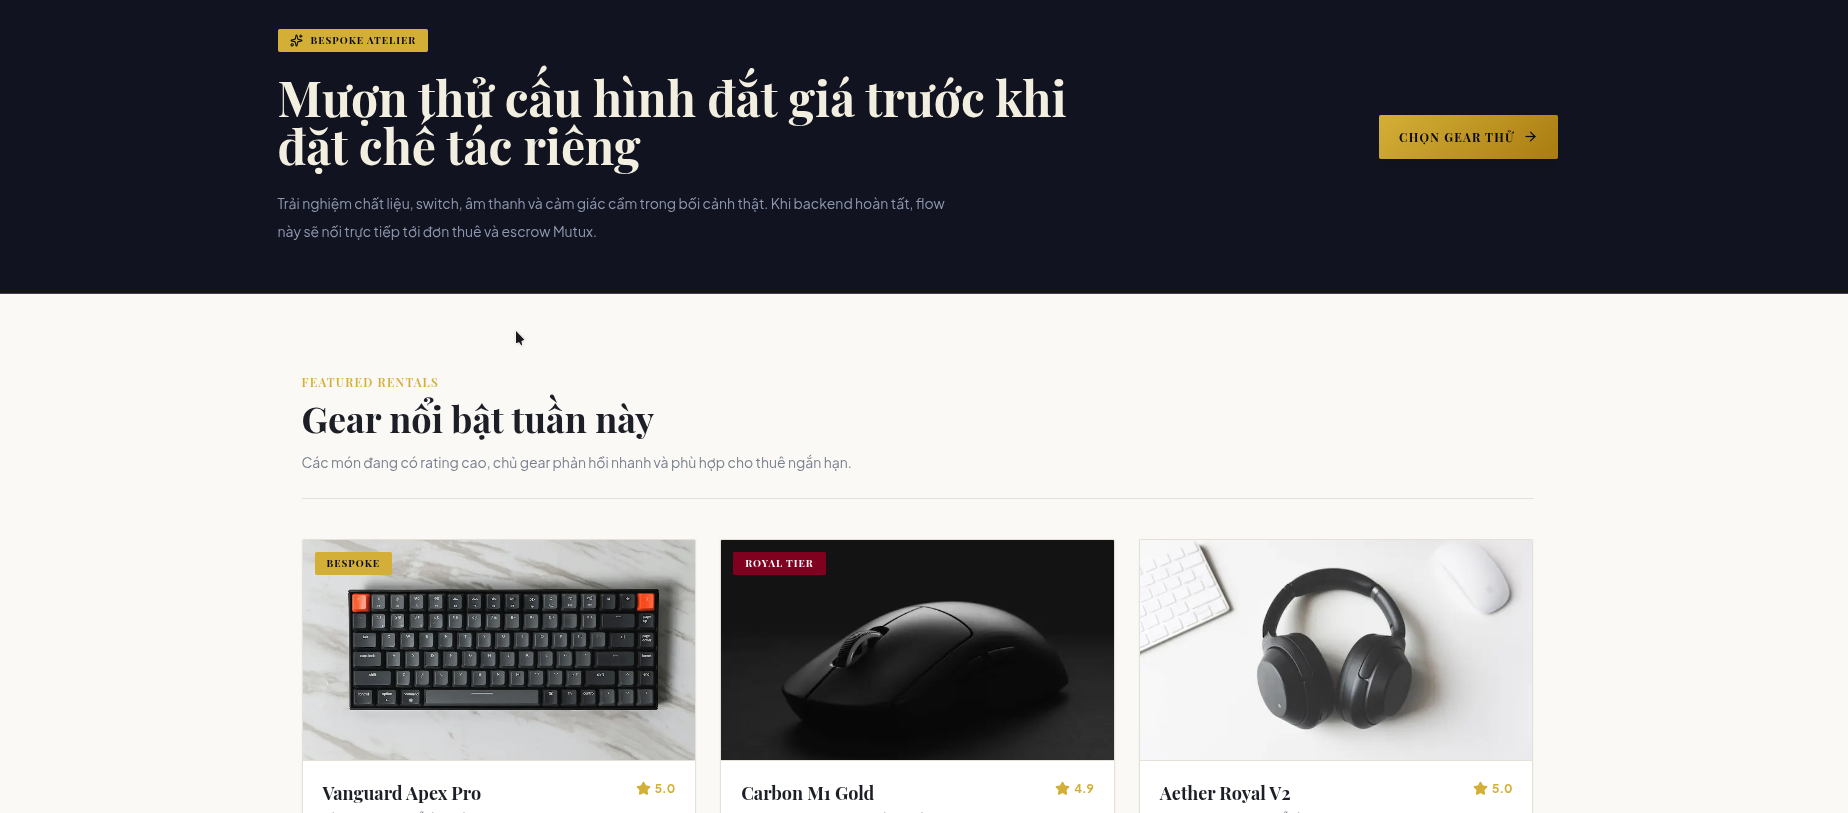
\includegraphics[width=1\textwidth]{../PA2/img/mvp/frontpage3.png}
    
    \caption{Trang chủ của Mutux}
    \label{fig:my_image}
\end{figure}

\begin{figure}[H]
    \centering 
    
    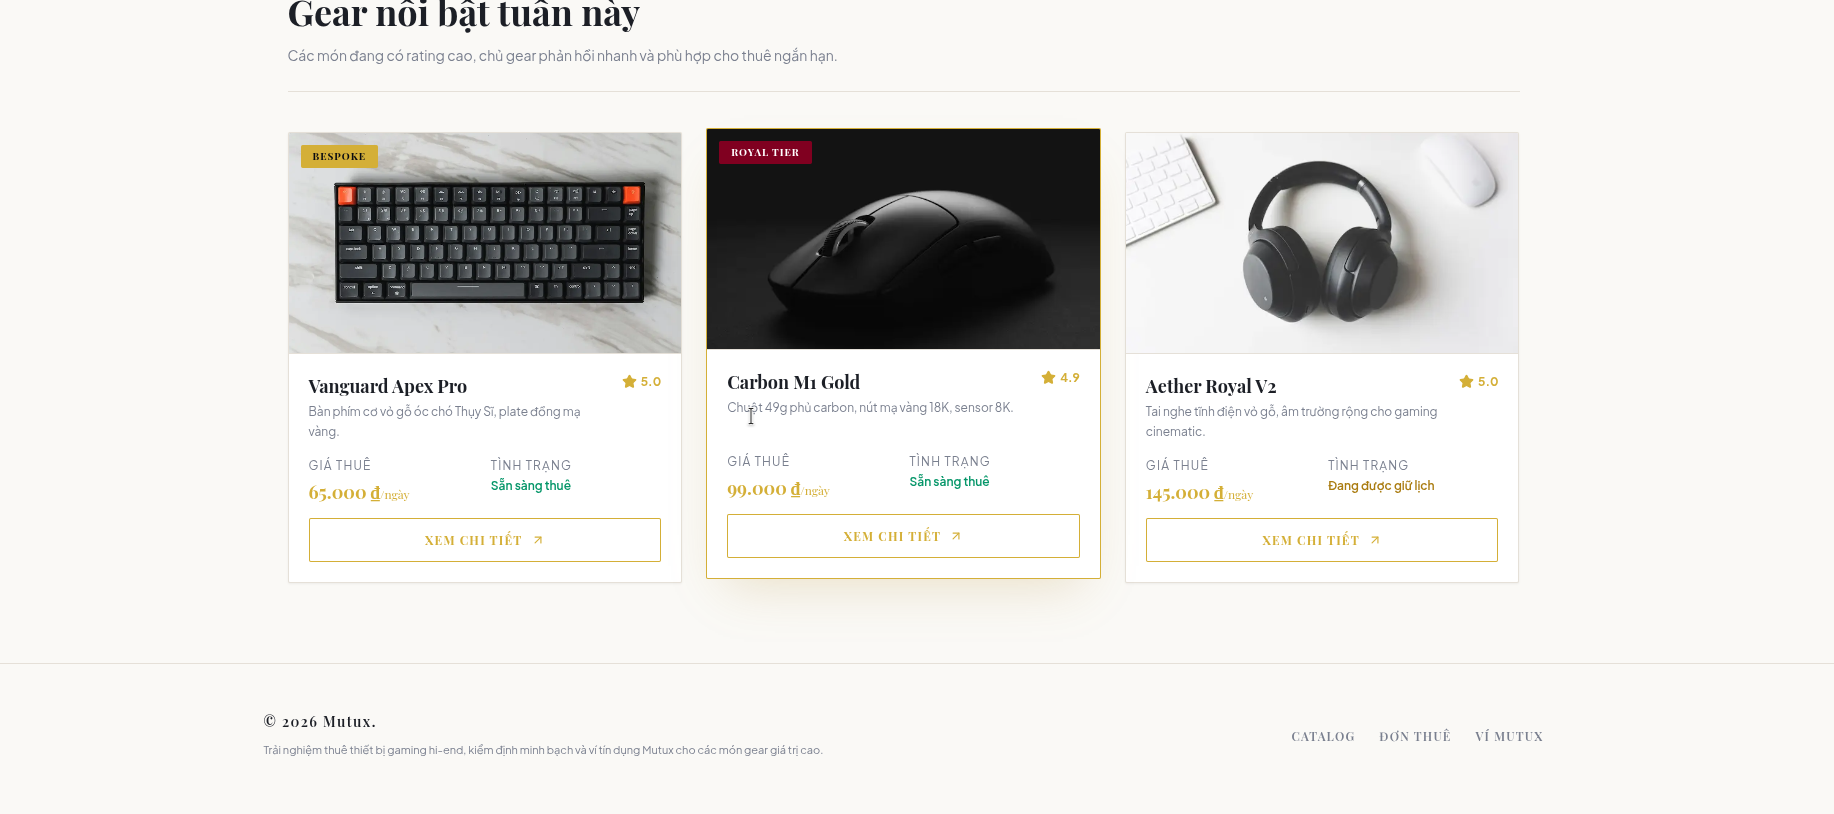
\includegraphics[width=1\textwidth]{../PA2/img/mvp/frontpage4.png}
    
    \caption{Trang chủ của Mutux}
    \label{fig:my_image}
\end{figure}

Tiếp đến, người dùng có thể vào mục \textbf{Sản phẩm} để xem danh mục các sản phẩm đang được cho thuê trên sàn.


\begin{figure}[H]
    \centering 
    
    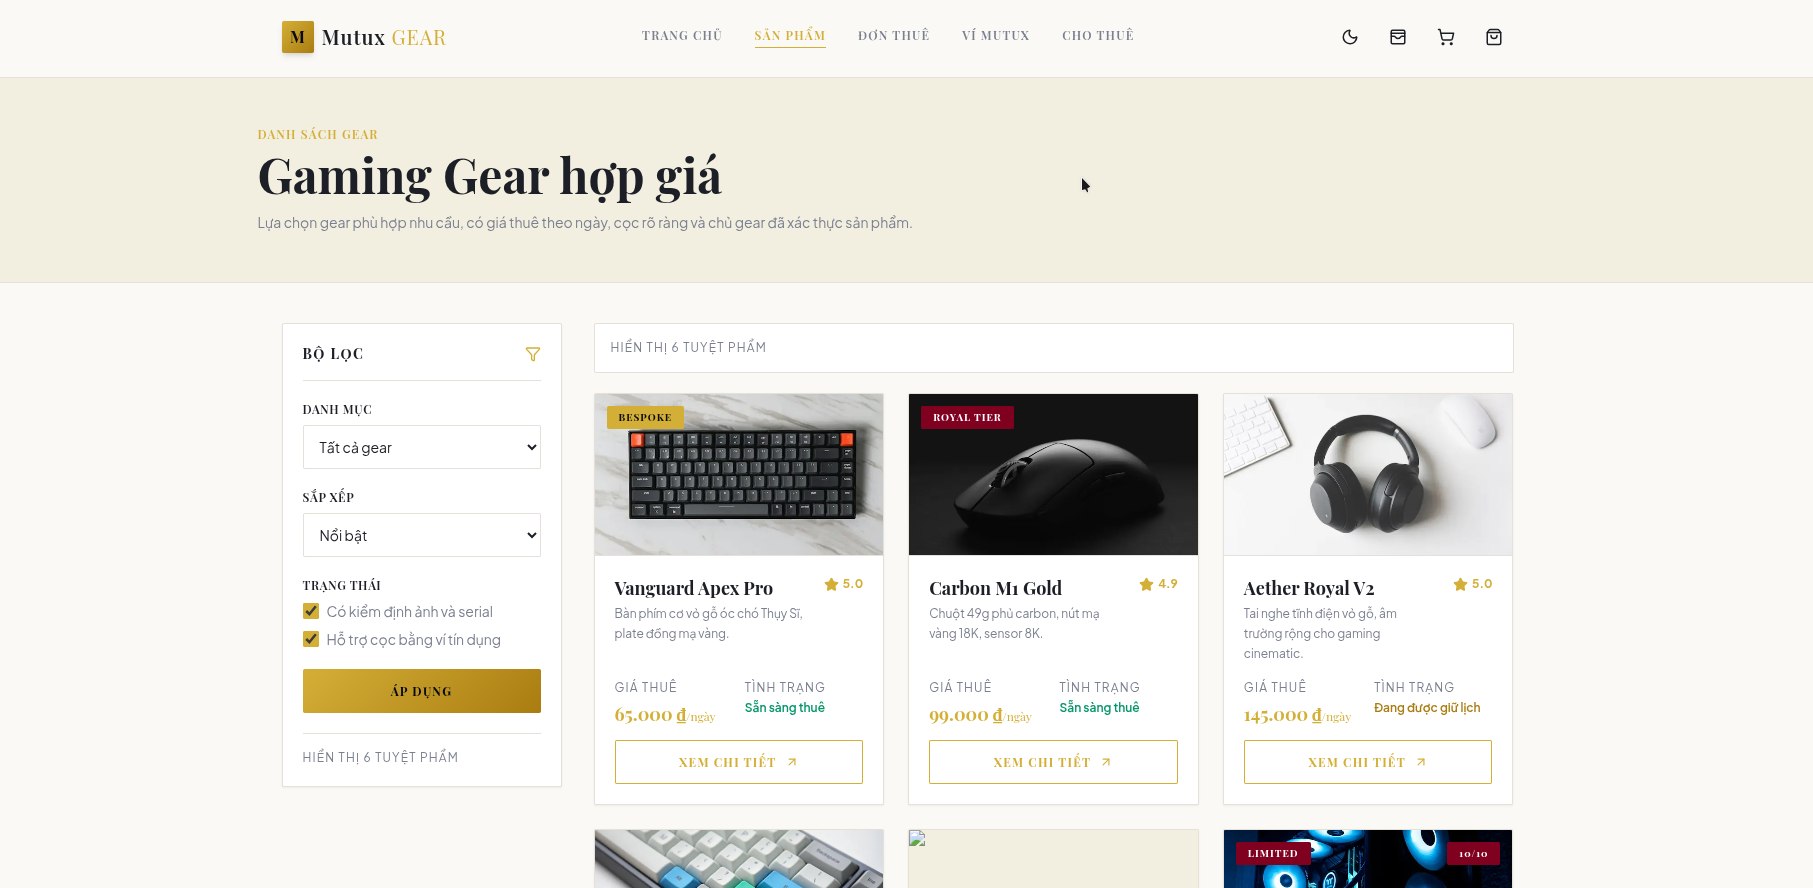
\includegraphics[width=1\textwidth]{../PA2/img/mvp/listgear1.png}
    
    \caption{Danh sách sản phẩm trên sàn Mutux}
    \label{fig:my_image}
\end{figure}

Ở tại đây, người dùng có thể filter được theo danh mục mà mình muốn


\begin{figure}[H]
    \centering 
    
    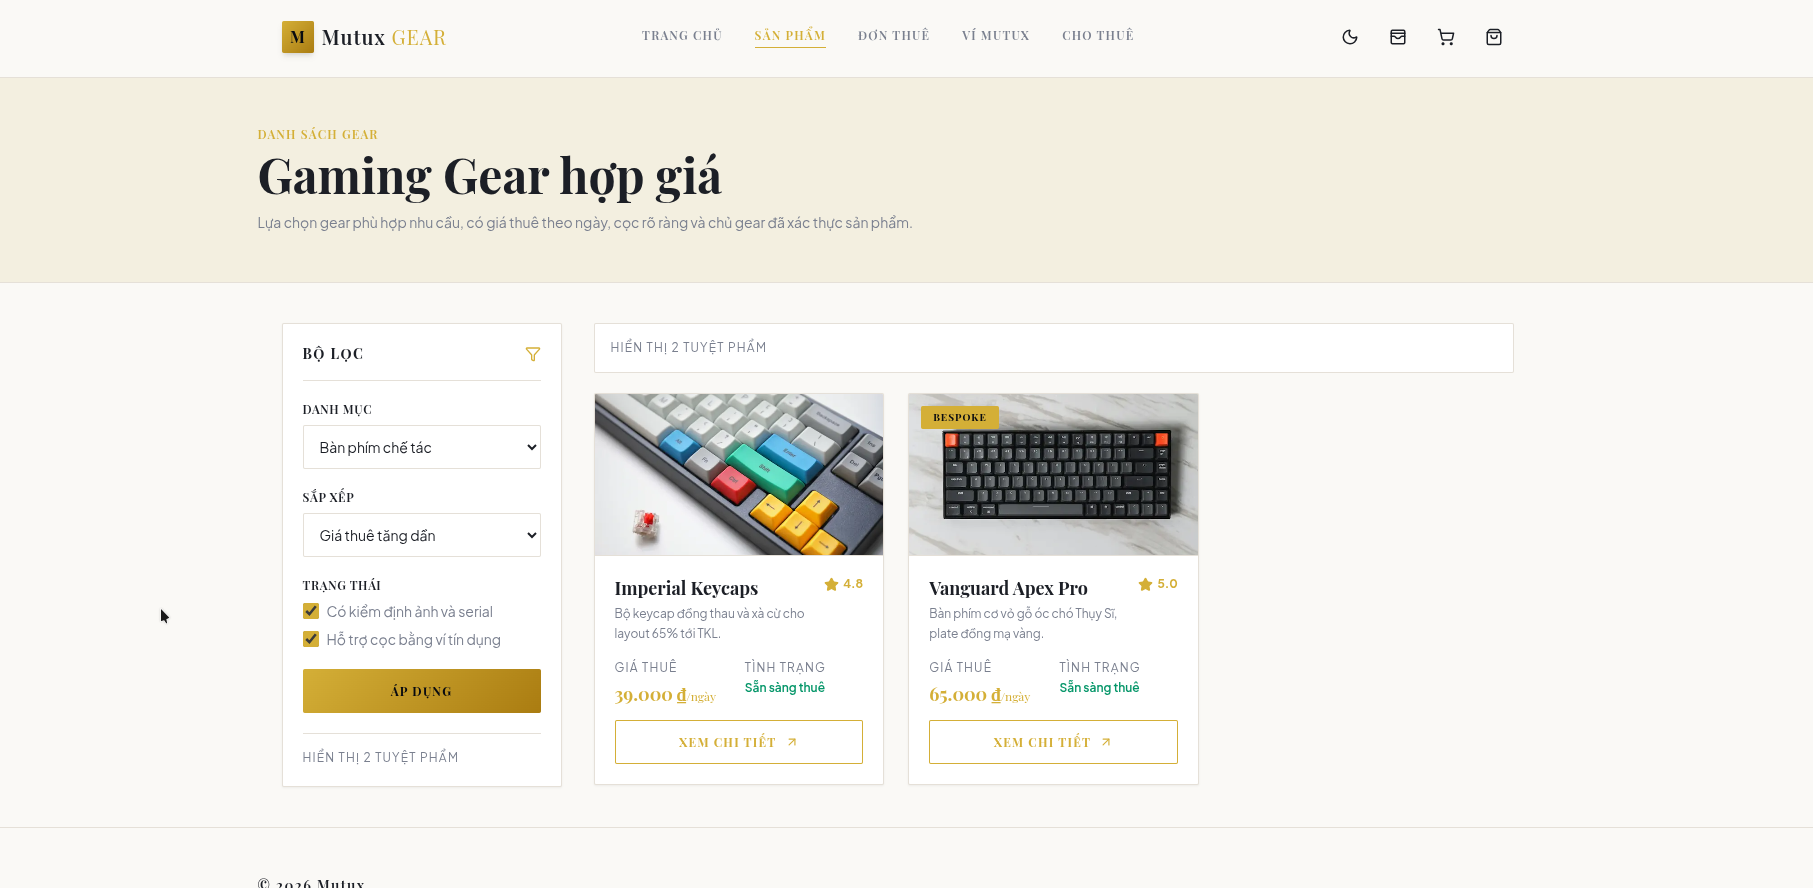
\includegraphics[width=1\textwidth]{../PA2/img/mvp/listgear-filter.png}
    
    \caption{Filter theo mục đích của người dùng}
    \label{fig:my_image}
\end{figure}

Sau đó, người muốn thuê chọn sản phẩm mình mong muốn để xem chi tiết

\begin{figure}[H]
    \centering 
    
    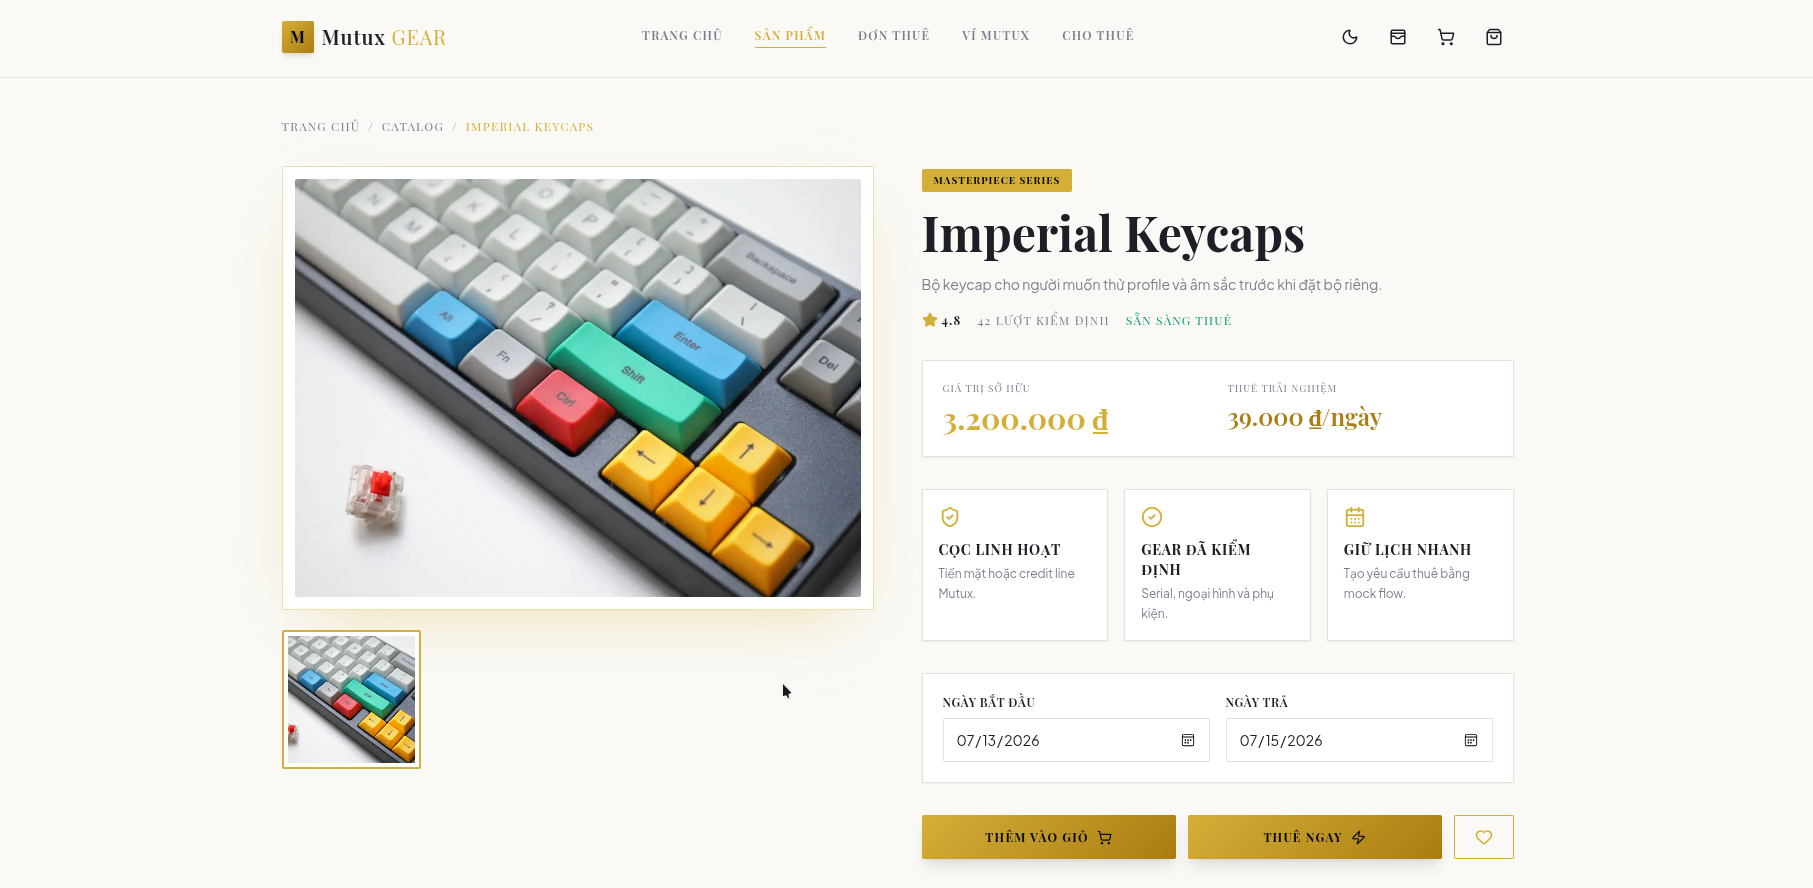
\includegraphics[width=1\textwidth]{../PA2/img/mvp/detailgear.png}

    \caption{Trang detail của sản phẩm}
    \label{fig:my_image}
\end{figure}

Tại đây, người dùng có thể chọn ngày bắt đầu đến ngày kết thúc thuê sản phẩm, sau đó, có thể chọn thêm vào giỏ hàng để tiếp tục xem các sản phẩm khác, hoặc tiến hành thanh toán ngay.


\begin{figure}[H]
    \centering 
    
    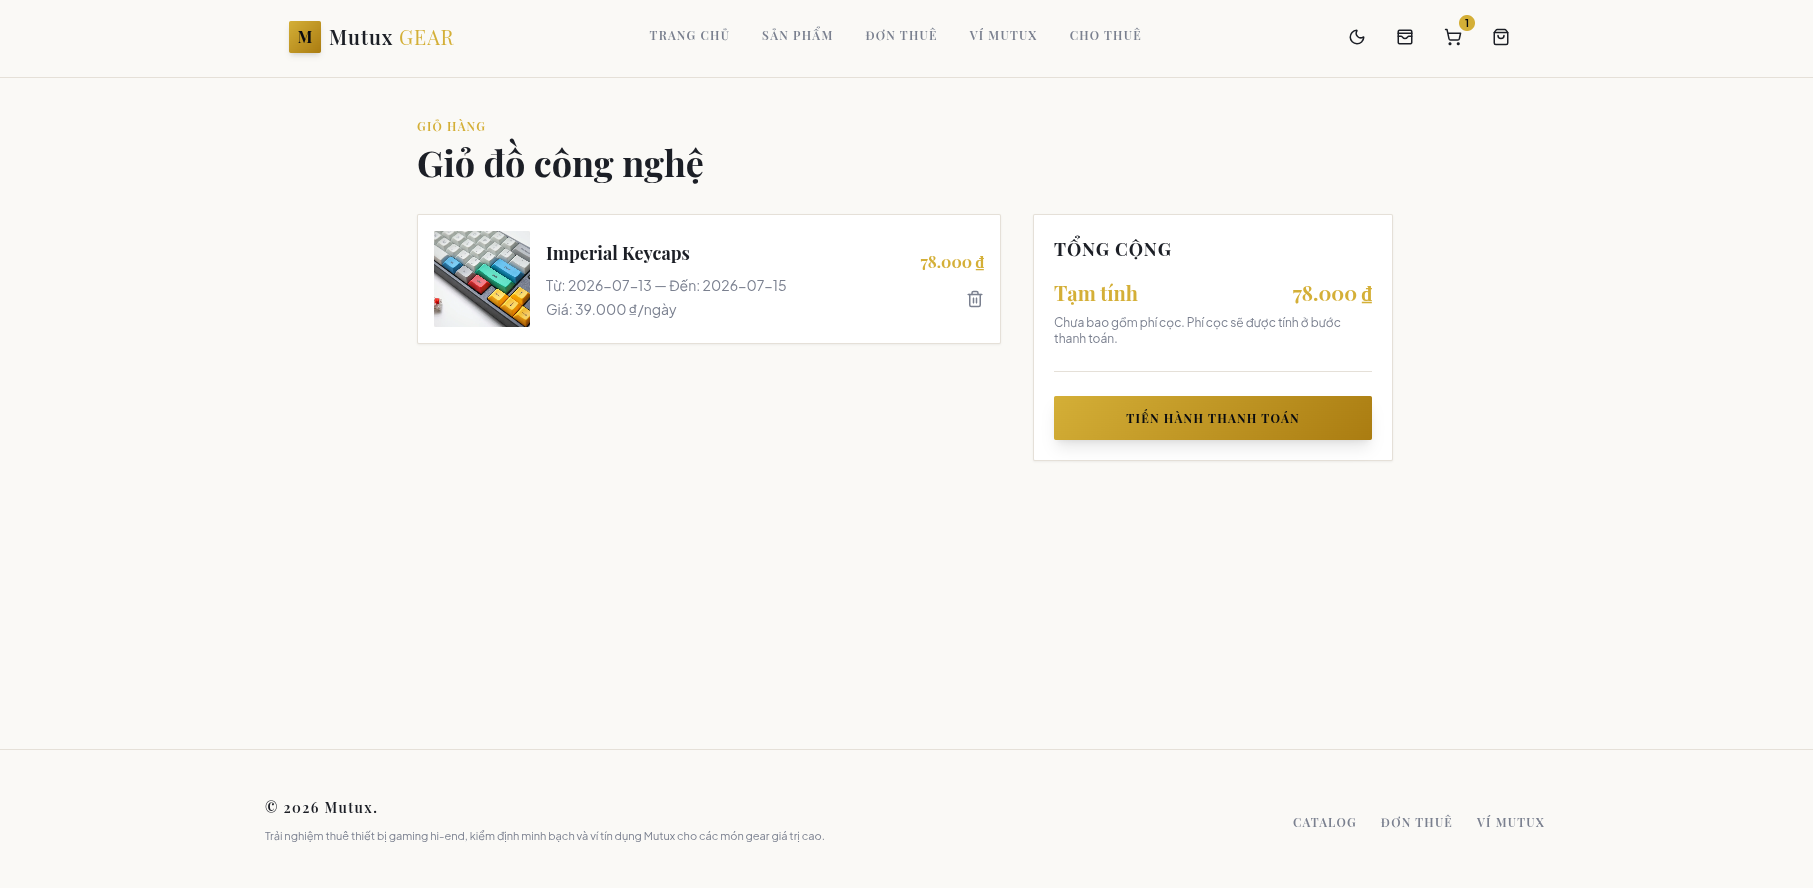
\includegraphics[width=1\textwidth]{../PA2/img/mvp/cart.png}

    \caption{Giỏ hàng sản phẩm}
    \label{fig:my_image}
\end{figure}


\begin{figure}[H]
    \centering 
    
    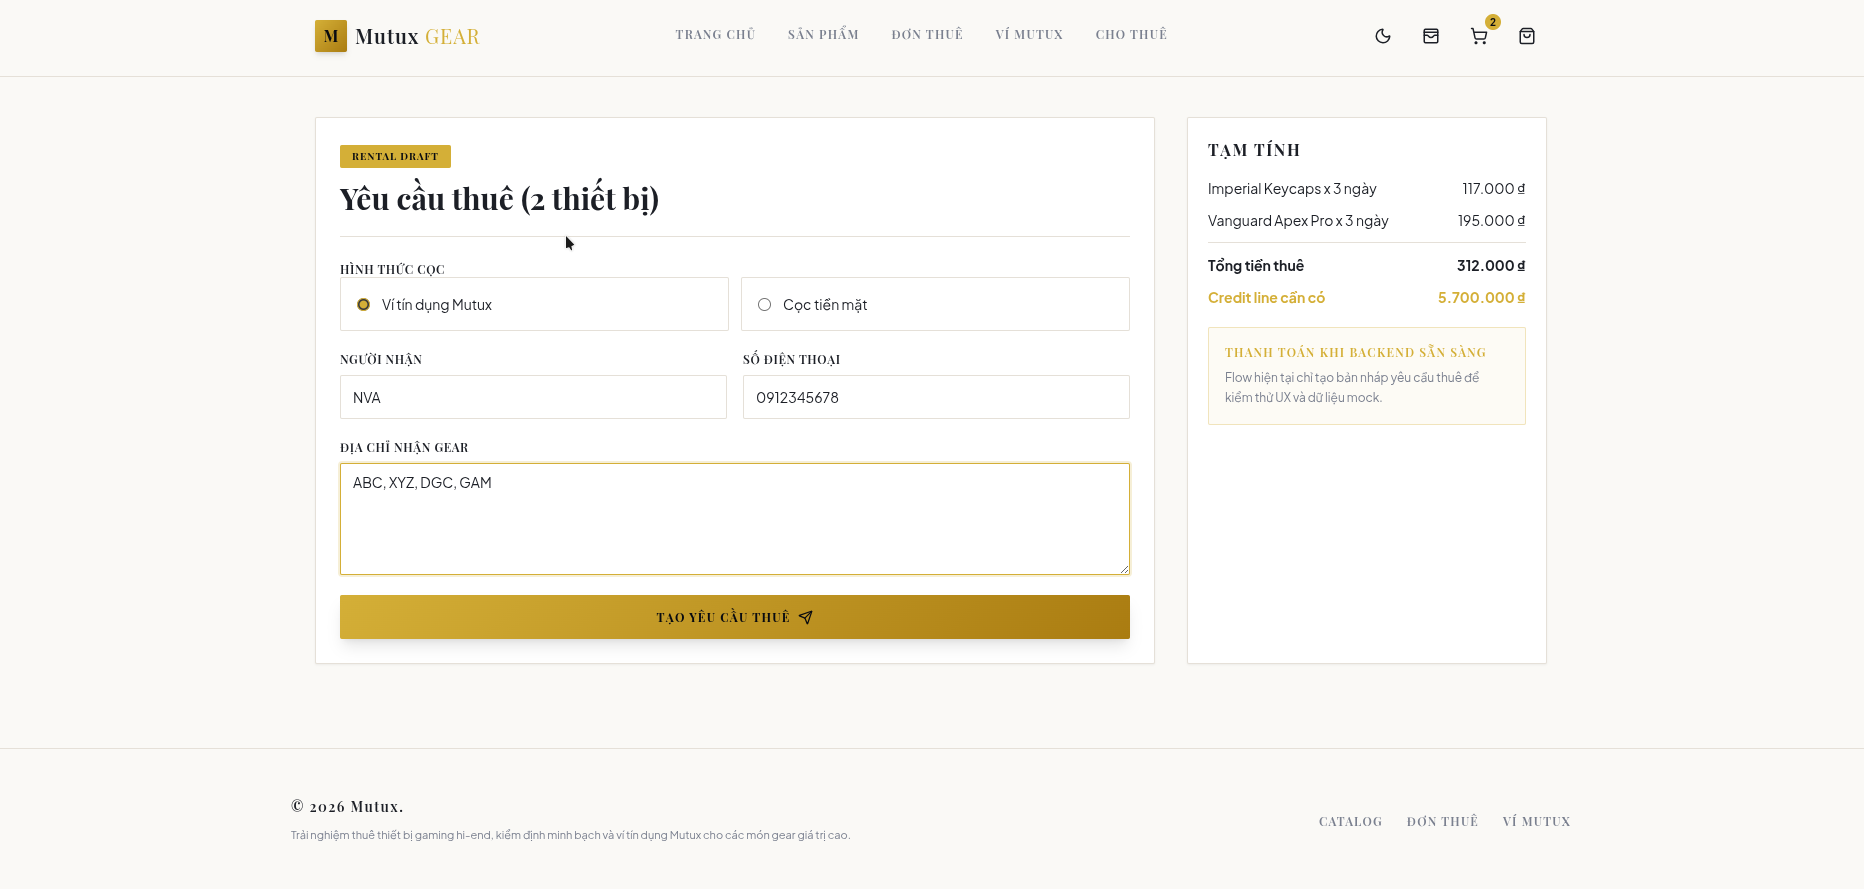
\includegraphics[width=1\textwidth]{../PA2/img/mvp/payment.png}

    \caption{Tiến hành thanh toán}
    \label{fig:my_image}
\end{figure}

Tại bước thanh toán, người dùng điền thông tin cá nhân đầy đủ của mình cho việc vận chuyển, bên cạnh đó chọn 2 phương thức thanh toán là cọc theo tiền mặt hoặc cọc theo ví Mutux của hệ thống. Sau khi nhấn \textbf{"Tạo yêu cầu thuê"} thì việc đặt thuê sản phẩm đã kết thúc.

Người dùng sau đó có thể xem các thông tin liên quan đến bản thân như dashboard của ví Mutux hoặc tổng hợp đơn hàng đã đặt
\begin{figure}[H]
    \centering 
    
    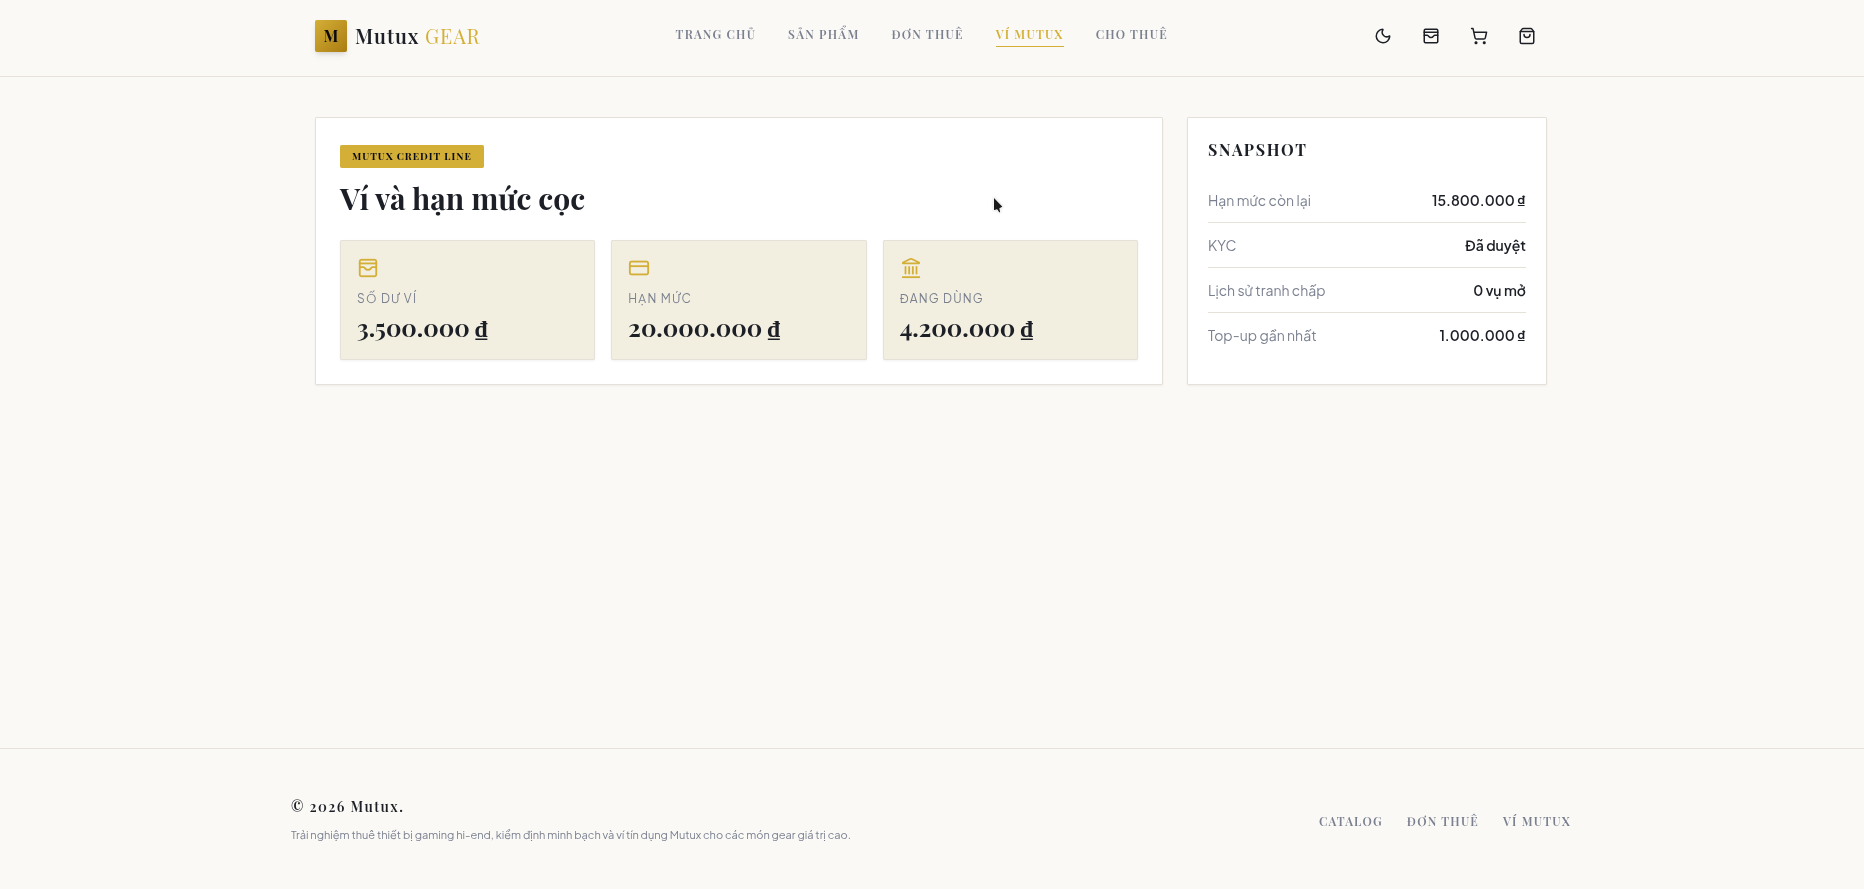
\includegraphics[width=1\textwidth]{../PA2/img/mvp/wallet.png}

    \caption{Dashboard quản lý ví Mutux}
    \label{fig:my_image}
\end{figure}


\begin{figure}[H]
    \centering 
    
    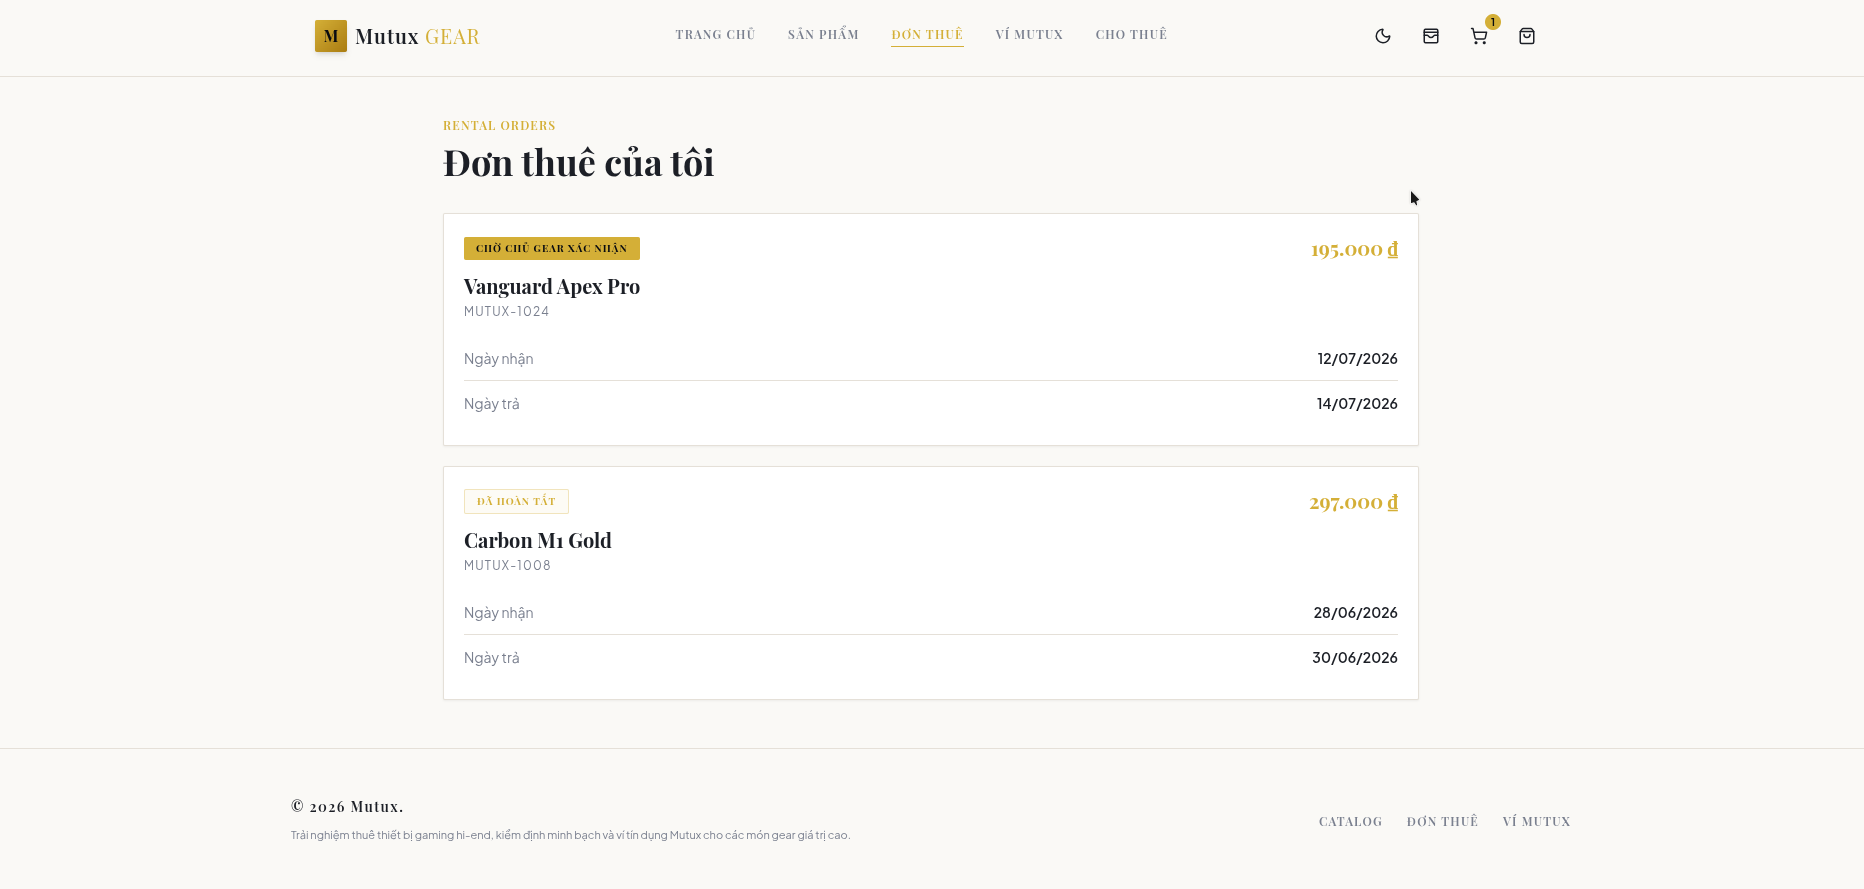
\includegraphics[width=1\textwidth]{../PA2/img/mvp/order.png}

    \caption{Tổng hợp đơn hàng đã thực hiện}
    \label{fig:my_image}
\end{figure}

Còn với bên người cho thuê, sau khi đăng nhập thì họ cũng có dashboard riêng để quản lý các thiết bị mình đã đăng lên. Tại đây họ có thể xem hoặc thực hiện các công đoạn liên quan đến CRUD cho các sản phẩm của mình.


\begin{figure}[H]
    \centering 
    
    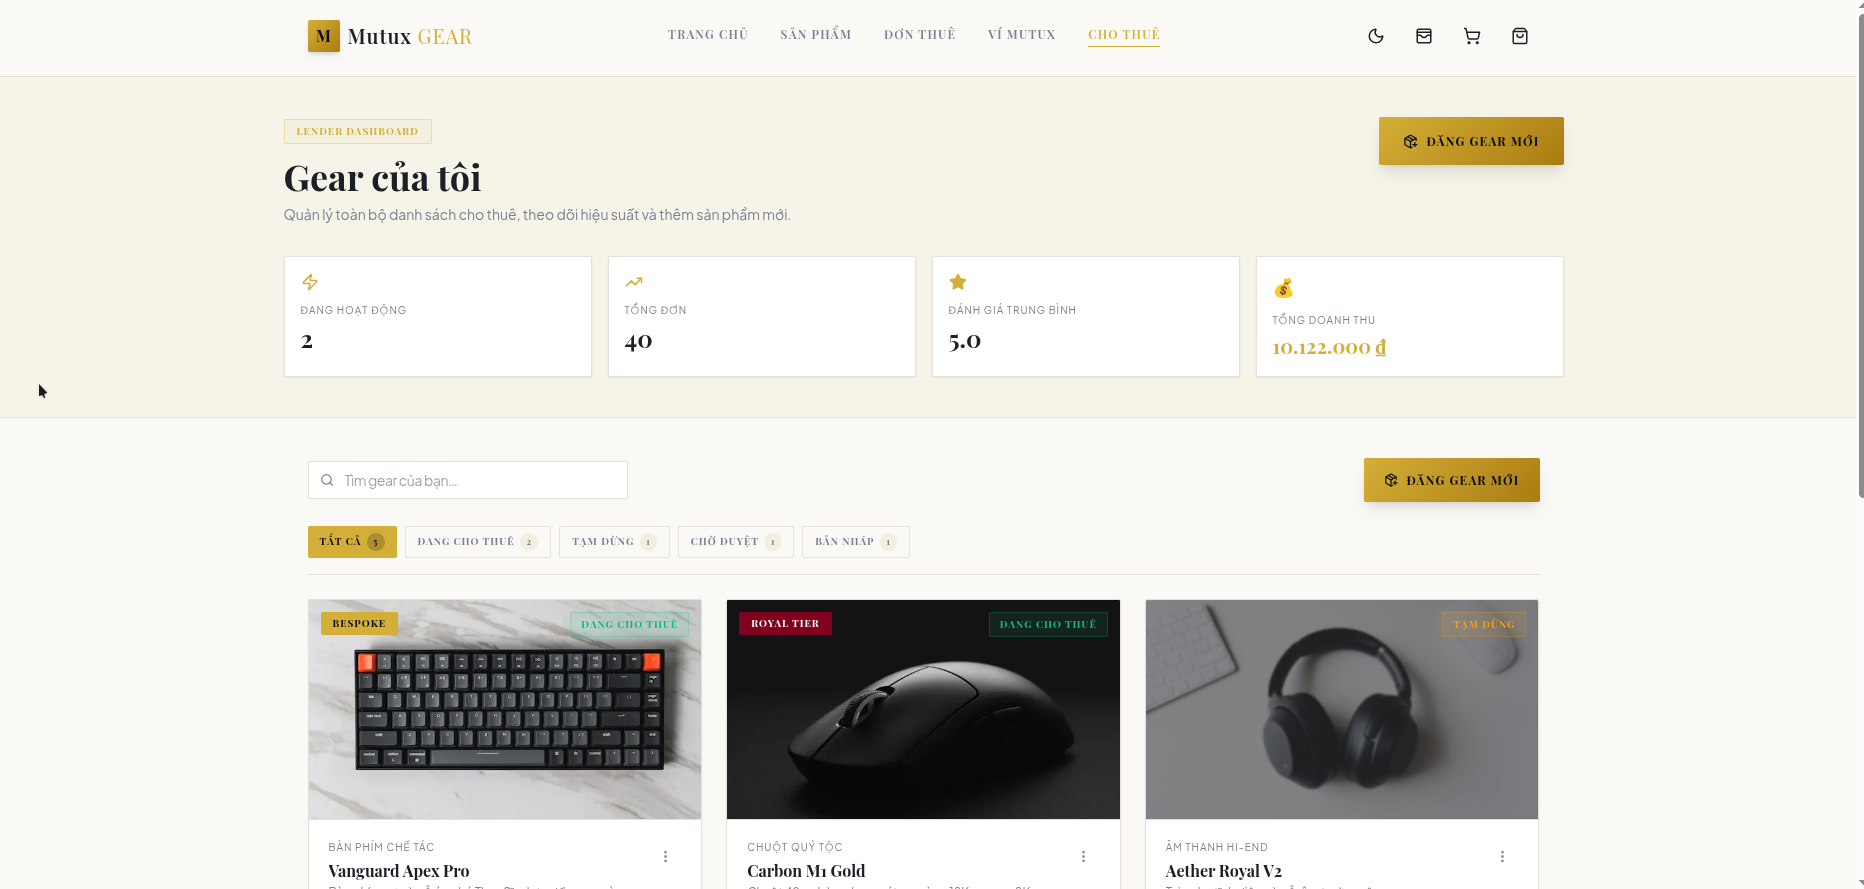
\includegraphics[width=1\textwidth]{../PA2/img/mvp/lender-dashboard.png}

    \caption{Dashboard của người cho thuê gear}
    \label{fig:my_image}
\end{figure}


\begin{figure}[H]
    \centering 
    
    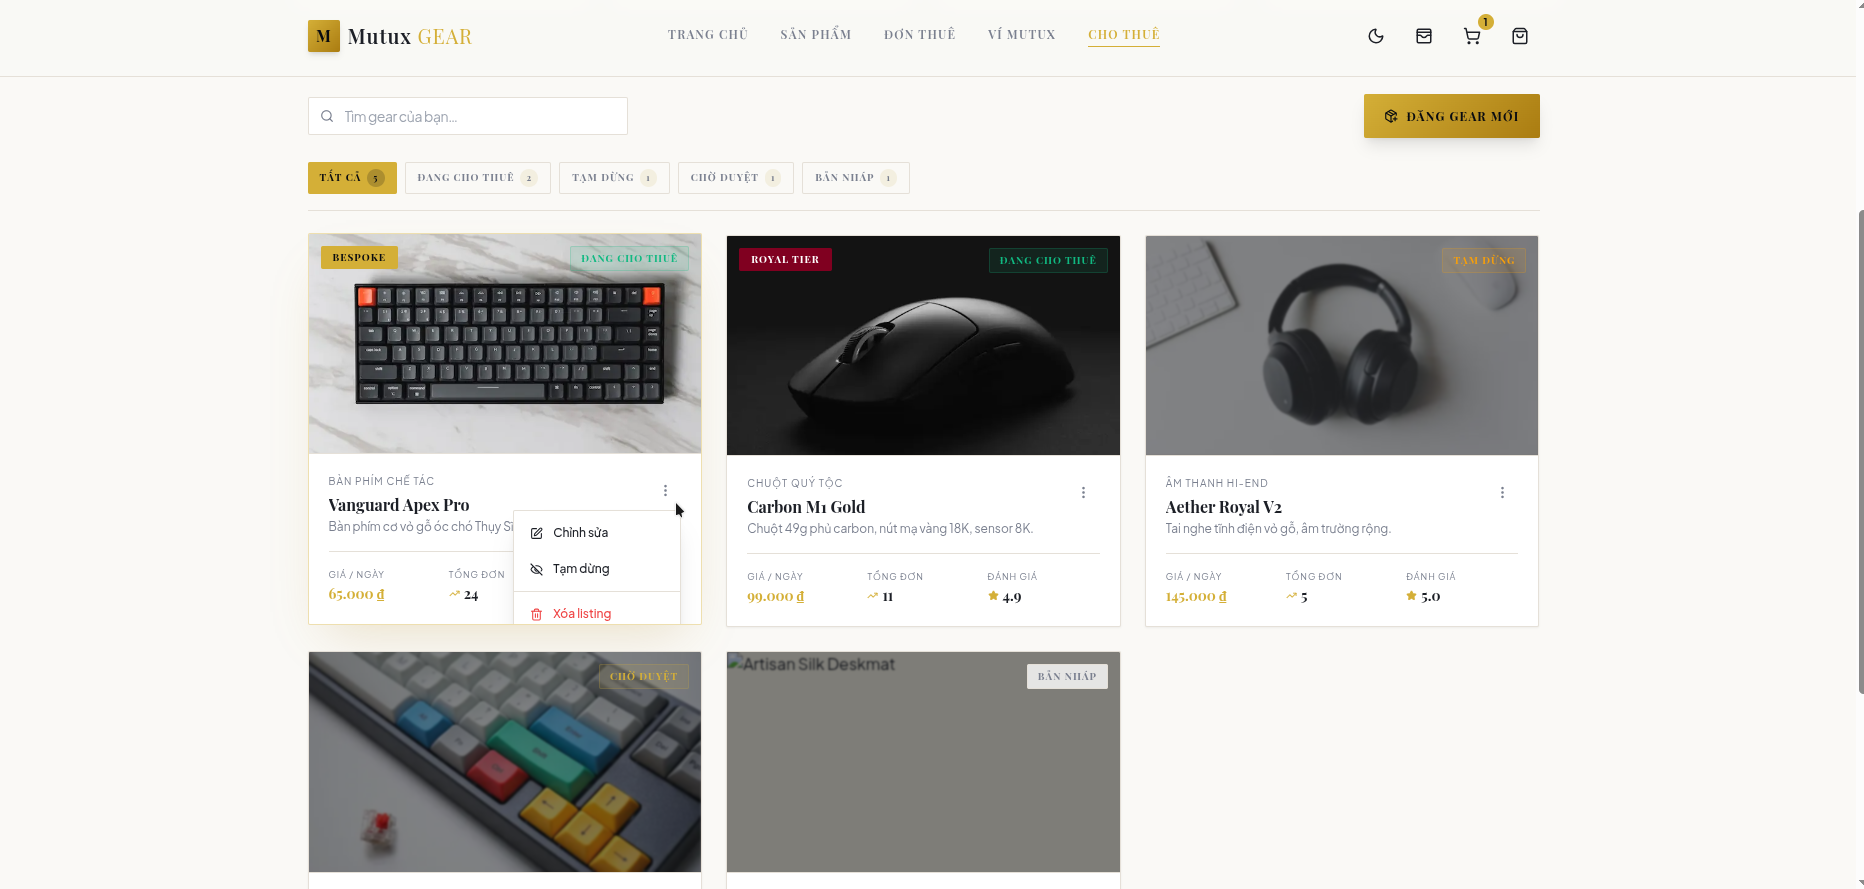
\includegraphics[width=1\textwidth]{../PA2/img/mvp/lender crud.png}

    \caption{CRUD sản phẩm đã đăng lên}
    \label{fig:my_image}
\end{figure}


Với sản phẩm mà người cho thuê muốn đăng lên mới, họ sẽ cần hoàn thành form đăng ký sản phẩm như sau:


\begin{figure}[H]
    \centering 
    
    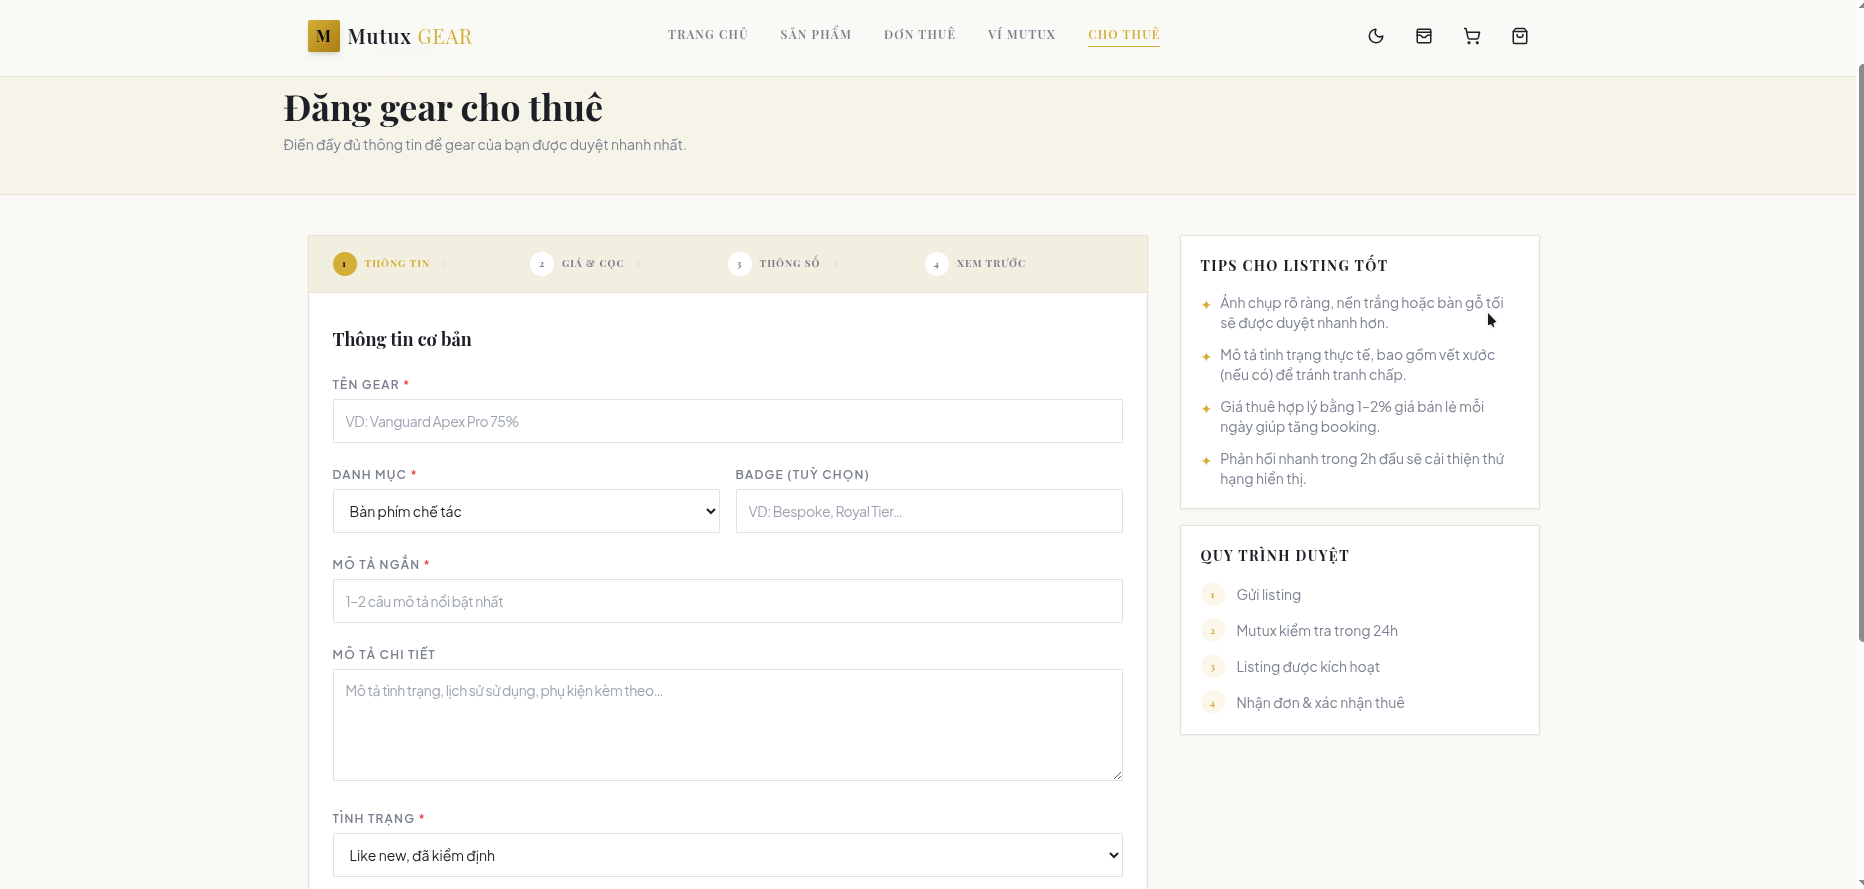
\includegraphics[width=1\textwidth]{../PA2/img/mvp/upload gear 1.png}

    \caption{Điền thông tin cơ bản của sản phẩm}
    \label{fig:my_image}
\end{figure}

\begin{figure}[H]
    \centering 
    
    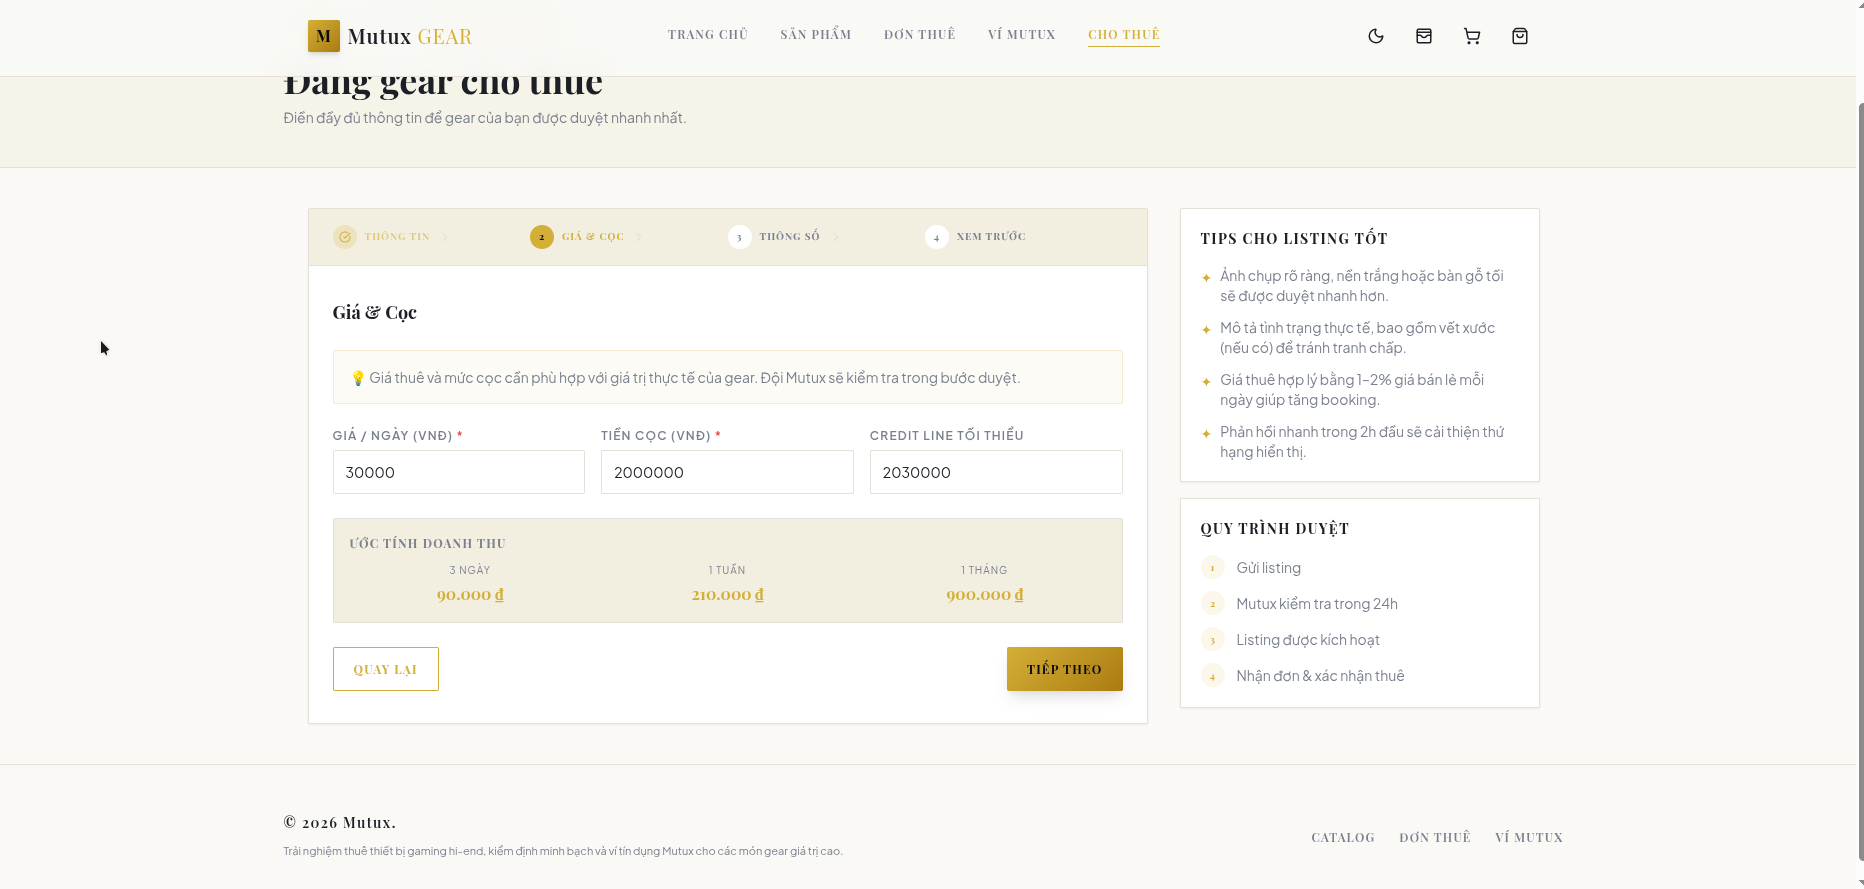
\includegraphics[width=1\textwidth]{../PA2/img/mvp/upload gear 2.png}

    \caption{Điền thông tin về giá sản phẩm}
    \label{fig:my_image}
\end{figure}

\begin{figure}[H]
    \centering 
    
    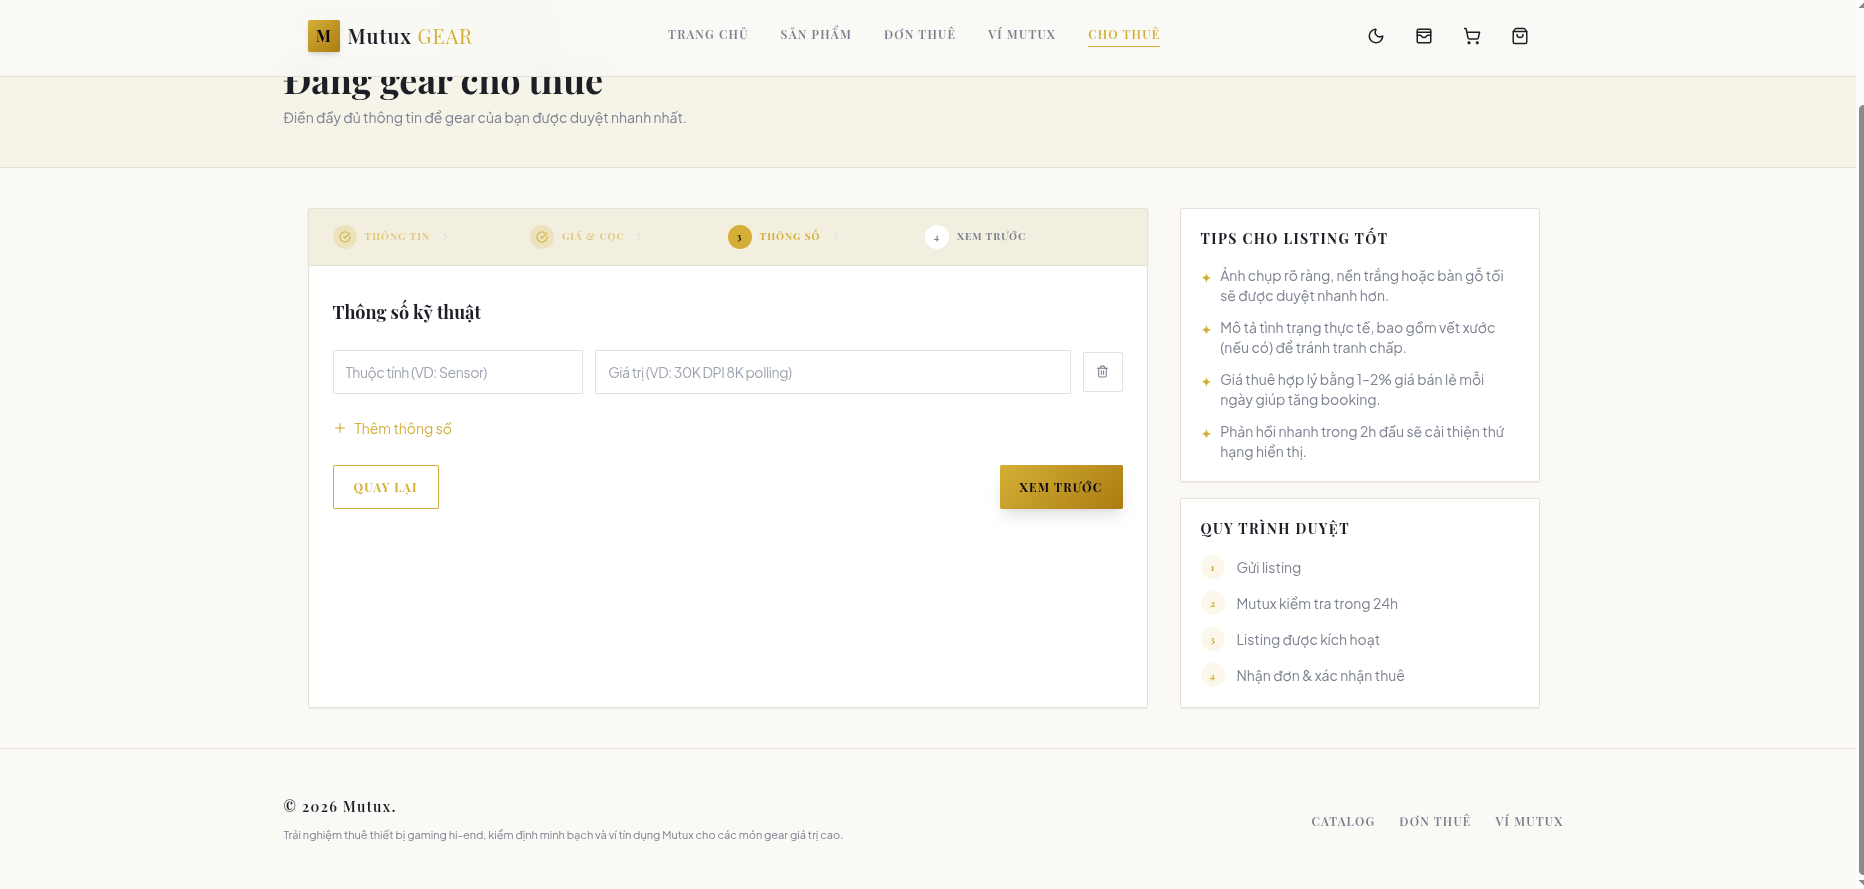
\includegraphics[width=1\textwidth]{../PA2/img/mvp/upload gear 3.png}

    \caption{Hoàn thành các thông tin kĩ thuật nếu có}
    \label{fig:my_image}
\end{figure}


\begin{figure}[H]
    \centering 
    
    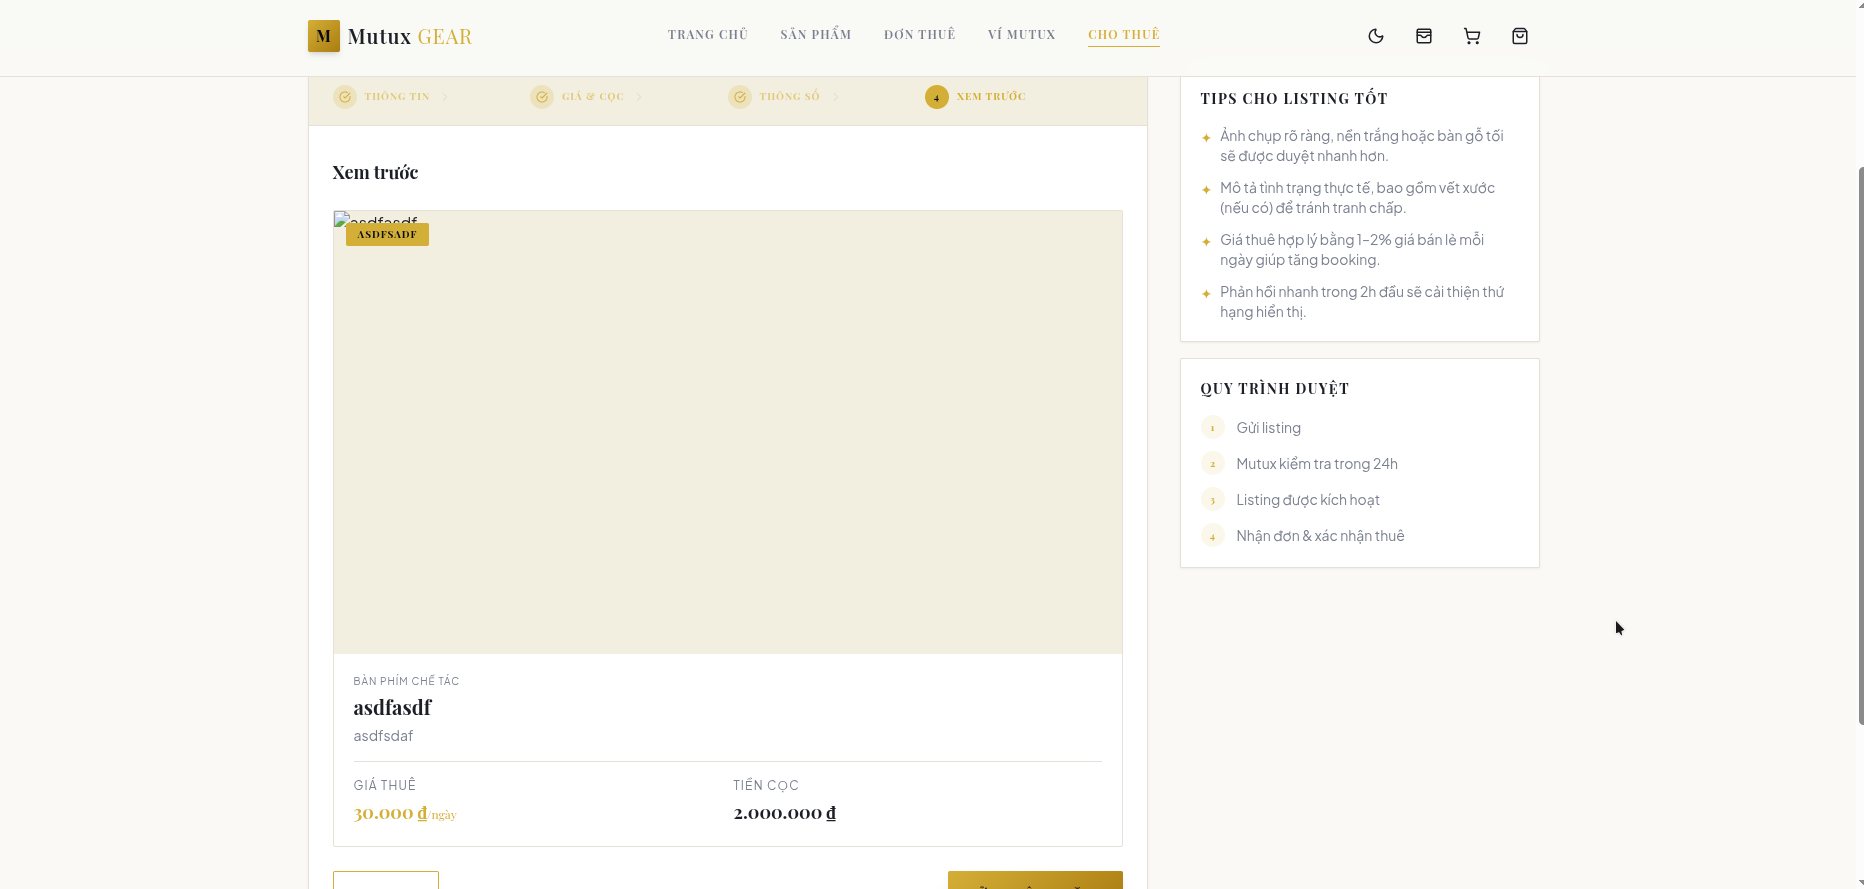
\includegraphics[width=1\textwidth]{../PA2/img/mvp/upload gear 4.png}

    \caption{Xem lại sản phẩm mình đã đăng lên}
    \label{fig:my_image}
\end{figure}


\begin{figure}[H]
    \centering 
    
    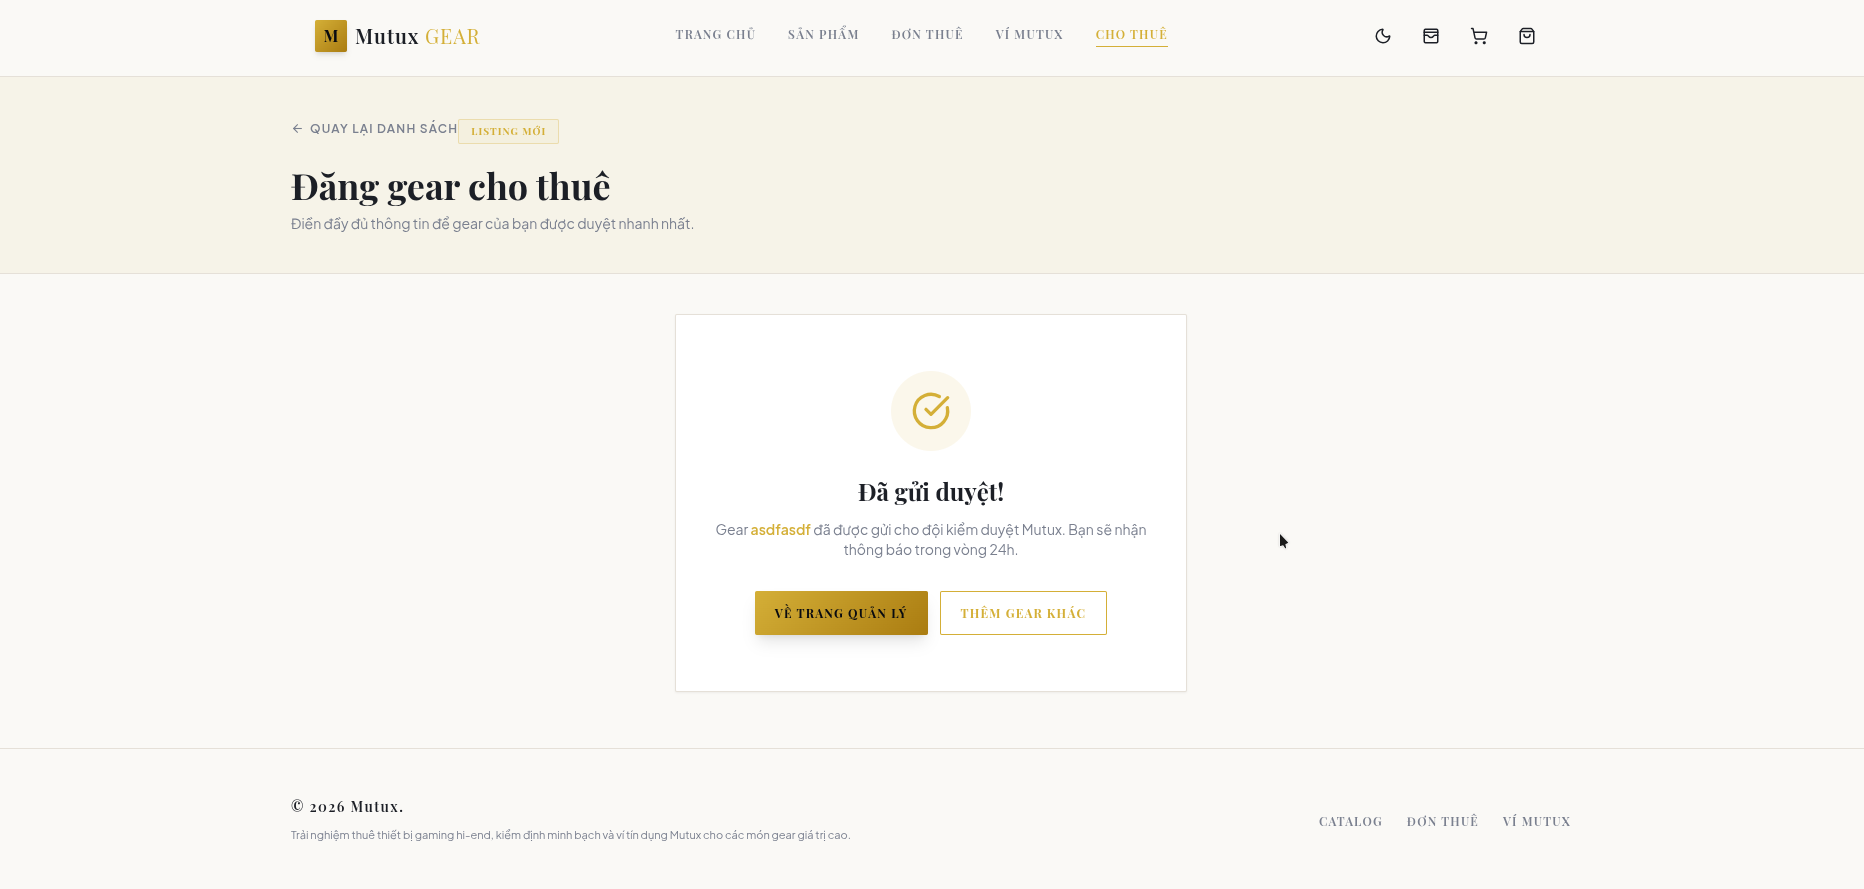
\includegraphics[width=1\textwidth]{../PA2/img/mvp/upload gear 5.png}

    \caption{Hoàn thành việc đăng sản phẩm lên sàn}
    \label{fig:my_image}
\end{figure}

Trên đây là UI cơ bản về luồng hoạt động quan trọng của Mutux, các UI quan trọng hơn cùng với MVP hoàn chỉnh sẽ được phát triển trong các giai đoạn tiếp theo.

